\documentclass[12pt, twoside]{book}

% Elenco dei packages utilizzati
\usepackage[a4paper,width=150mm,top=25mm,bottom=25mm,bindingoffset=6mm]{geometry}
\usepackage[utf8]{inputenc}
\usepackage[T1]{fontenc}
\usepackage[italian]{babel}
\usepackage{subcaption}
\usepackage{graphicx}
\usepackage{fancyhdr}
\usepackage{float}
\usepackage{color}
\usepackage[nottoc]{tocbibind}
\usepackage{emptypage}
\usepackage[hidelinks]{hyperref}
\usepackage{titlesec}
\usepackage{amssymb}
\usepackage[sorting=none,backend=bibtex]{biblatex}
\usepackage{csquotes}
\usepackage{pdfpages}
\usepackage{amsmath}
\usepackage{placeins}
\usepackage{hyperref}
\usepackage{footnote}
\usepackage{import}
\usepackage{listings}
\lstset{
basicstyle=\small\ttfamily,
columns=flexible,
breaklines=true
}
% \usepackage{minted}
\usepackage{xcolor}

% page styles
\pagestyle{fancy}
\definecolor{LightGray}{gray}{0.9}
% \usemintedstyle{colorful}

% Bibliography
\addbibresource{./bibliography/bibliography.bib}

\begin{document}


\includepdf{chapters/0.frontpage/front.pdf}

\cleardoublepage

\tableofcontents

\phantomsection
\listoffigures

\chapter*{Introduzione}
\chaptermark{Introduzione}
\addcontentsline{toc}{chapter}{Introduzione}
Negli ultimi decenni, la crescente richiesta di servizi e applicazioni online ha portato ad un'esplosione dello sviluppo
delle tecnologie web. Questo cambiamento è stato reso possibile dall'aumento dell'ubiquità dei dispositivi connessi a
Internet, che rendono l'accesso ai servizi web sempre più immediato, semplice e alla portata di tutti. Di conseguenza,
le tecnologie e le applicazioni che garantiscono questi servizi devono essere in grado di rispondere in modo efficiente
a volumi di dati e utenti sempre maggiori. In questo scenario, il cloud computing rappresenta un elemento essenziale per
la gestione di applicazioni distribuite, ovvero applicazioni suddivise in più componenti spesso eterogenei, sia per
composizione che locazione fisica. 

Il cloud computing è un modello di erogazione di servizi che consente di gestire l'infrastruttura informatica necessaria
per rendere disponibili applicazioni, dati e servizi online in modo rapido, efficiente e flessibile. Grazie al cloud
computing, le risorse informatiche come server, storage e software possono essere facilmente scalate per rispondere alle
esigenze delle organizzazioni e degli utenti finali, consentendo un accesso sicuro e veloce ai servizi e alle
applicazioni da qualsiasi dispositivo connesso a Internet. La rapidità e velocità con cui il cloud computing eroga
questi servizi è data dalle tecnologie che lo compongono. \\
In questo contesto andremo a discutere di una emergente tecnologia, chiamata \textbf{WASI (WebAssembly System
Interface)}\footnote{\url{https://wasi.dev/}} e come questa possa essere considerata la terza ondata del cloud
computing\cite{cloudcomputing-thirdwave}. Grazie a WASI, è possibile eseguire applicazioni in un ambiente isolato e
sicuro, senza la necessità di dover conoscere il sistema operativo sottostante. È stato progettato per essere altamente
portabile, consentendo alle applicazioni di essere eseguite in modo efficiente su qualsiasi piattaforma. \\
Nasce e si sviluppa sopra ad una tecnologia già esistente: \textbf{WebAssembly} (o \textbf{Wasm}). Quest'ultima è
un'innovativa tecnologia nata con l'obiettivo di migliorare le prestazioni delle applicazioni web \textbf{sul browser}.
È stata progettata con l'intento di superare le limitazioni poste da Javascript. In particolare, si propone di essere
veloce, efficiente e portabile, oltre che retro-compatibile con le tecnologie già esistenti. Va notato che WebAssembly
non è pensato per sostituire JavaScript, ma piuttosto per migliorare le aree in cui quest'ultimo presenta alcune lacune:
come il rendering 3D, il video editing, giochi in-browser e così via. \\
WASI eredita tutte queste caratteristiche da Wasm e le utilizza per lo sviluppo di applicazioni \textbf{al di fuori} dei
browser. \\\\
Di seguito andremo ad approfondire WASI ed esporremo come rappresenti una tecnologia estremamente promettente per il
futuro nell'ambito del cloud computing. Si partirà affrontando l'argomento da un punto di vista generale, andando a
definire le motivazioni storiche che hanno portato alla sua ideazione, il suo funzionamento e lo stato dell'arte della
tecnologia. Lo si metterà a confronto con le soluzioni esistenti, in particolare affrontando le sue principali
somiglianze e differenze con il modello a container, estremamente popolare al giorno d'oggi e con il suo predecessore,
le macchine virtuali. Si studieranno le principali caratteristiche ereditate  da Wasm ponendo particolare attenzione
alla loro implementazione fuori dal browser da un punto di vista tecnico. Tra queste caratteristiche ritroviamo:
\begin{itemize}
    \item \textbf{efficienza}, dato il suo formato binario di piccole dimensioni, simile al linguaggio macchina
    \item \textbf{portabilità}, grazie alla possibilità di essere eseguito su molteplici sistemi e architetture allo
    stesso modo mediante applicazioni dette runtime simili, per funzionamento, alla JVM di Java.
    \item \textbf{interoperabilità}, grazie al fatto che non è strettamente legato ad alcun linguaggio di programmazione
    specifico
    \item \textbf{sicurezza}, in quanto eseguito in ambiente sandbox secondo il modello capability-based
\end{itemize}

La spiegazione teorica sul funzionamento e sui vantaggi sfocerà in un'implementazione di un piccolo prototipo scritto in
linguaggio Rust basato su un'architettura a microservizi REST API in cui si andranno a mettere in pratica i concetti
visti in precedenza. Si andrà a valutare il deployment dell'applicazione e ad effettuare benchmark per valutarne i tempi
di risposta a livelli di carico differenti per simularne un caso d'uso reale. I risultati ottenuti saranno messi a
confronto con un'applicazione che propone le stesse funzionalità ma implementata con una diversa tecnologia.
\chapter{WASI}
\label{chap:wasi-in-depth}
L'obiettivo principale di WASI è fornire un set di API standard per WebAssembly, indipendenti dall'architettura
sottostante. Per raggiungere questo obiettivo è stato necessario creare, in prima istanza, un primo modulo su cui basare
tutti gli altri. Questo modulo è stato chiamato WASI-core e ha lo scopo di fornire le funzionalità di base per
l'ambiente di esecuzione, come la gestione dei file, delle reti e di essere generico in modo da poter essere utilizzato
in qualsiasi ambiente fuori dal browser. Al di fuori del contesto web, WebAssembly ha bisogno di una serie di API per
interagire con il sistema operativo sottostante, ovvero una libreria di sistema per Wasm. Questa libreria, chiamata
WASI-libc è in grado di fornire un ponte tra i moduli Wasm e le system call del sistema sottostante. È basata sullo
standard POSIX\cite{posix-standard}, in particolare su musl-libc\footnote{\url{http://musl.libc.org/}} ed utilizza le
funzioni di libpreopen\footnote{\url{https://github.com/musec/libpreopen}}.
% È basata sullo standard POSIX in particolare su musl-libc\footnote{\url{http://musl.libc.org/}}, un'implementazione
% dello standard POSIX costruita sulle system call di Linux ed utilizza le funzioni di
% libpreopen\footnote{\url{https://github.com/musec/libpreopen}}, un insieme di funzioni che consente solo l'uso di file
% descriptor già aperti in precedenza, prevenendo così la possibilità di aprire file descriptor direttamente. Questi
% file descriptor sono aperti dai runtime WASI e passati all'applicazione in un secondo momento, in modo da rispettare
% il capability-based security model. L'implementazione di WASI-libc non porta include funzioni come fork() o exec() in
% quanto complesse da sviluppare in ambito sandbox e al momento fuori dallo scope del progetto.

\section{WASI-libc}
WASI-libc\footnote{\url{https://github.com/WebAssembly/WASI/blob/main/legacy/preview1/docs.md}} è una libreria che
definisce un'interfaccia C standard per le system call necessarie a WebAssembly. È il ponte fondamentale che unisce i
moduli Wasm con il sottostante sistema operativo. L'obiettivo chiave della libreria è quello di fornire un set di
funzioni che si comportino come quelle dello standard POSIX, ma che siano implementate specificamente per WebAssembly
tra cui l'allocazione e la manipolazione della memoria, l'I/O dei file, la gestione delle stringhe, le funzioni
matematiche e così via. Essendo un'implementazione personalizzata, non include tutte le funzioni standard di POSIX. Ad
esempio funzioni come la fork() e l'exec() sono escluse in quanto complesse da implementare in ambito sandbox e
difficili da gestire secondo il modello capability-based. La libreria è basata su due altre librerie già esistenti: la
musl-libc e la libpreopen.
\subsection{Musl-libc}
Musl-libc è una libreria standard del linguaggio C che fornisce una serie di funzioni predefinite per semplificare lo
sviluppo di software. La libreria è stata progettata per essere leggera, efficiente e altamente portabile, ed è stata
sviluppata con un focus particolare sulla compatibilità POSIX. Si propone come un'alternativa più leggera e veloce
rispetto alla GNU C Library (glibc). Tra le funzionalità supportate da musl-libc vi sono la gestione della memoria, le
operazioni su stringhe, la gestione dei file, i socket di rete e la gestione dei processi.
\subsection{Libpreopen}
\label{sec:libpreopen}
Libpreopen è una libreria che fornisce un meccanismo per caricare in anticipo e intercettare le operazioni sui file in
un sistema operativo. Consente alle applicazioni di aprire i file utilizzando un insieme predefinito di regole e
percorsi, anziché il percorso effettivo sul filesystem. Libpreopen intercetta le chiamate di sistema relative, come
open(), stat() e opendir(), e le traduce in operazioni definite dalle applicazioni. Consente all'applicazione di
specificare un insieme di regole che definiscono come i file devono essere accessibili. Ad esempio, un'applicazione
potrebbe specificare che tutte le operazioni sui file dovrebbero essere eseguite in una directory o file system montato
specifico, o che determinati file dovrebbero essere in sola lettura o scrittura. Su questi concetti si basa il
capability-based security di WASI ed è perciò di fondamentale importanza per il suo funzionamento.
% \subsection{Perché è necessaria una libc?} È il mattoncino base fondamentale per l'interazione con il sistema
% operativo sottostante, in quanto fornisce le funzioni standard di base necessarie per lo sviluppo delle applicazioni.
% Senza una libreria standard come la libc, gli sviluppatori dovrebbero scrivere manualmente il codice per queste
% funzioni di basso livello, il che sarebbe molto laborioso e inefficiente. Si noti che la libc non è un requisito
% esclusivo di WASI, è la base su cui poggiano tutti i sistemi informatici moderni!

\section{La Portabilità}
Nell'introduzione abbiamo discusso del ruolo di WASI come standard che consente di eseguire il codice WebAssembly su
sistemi operativi e architetture diverse, in modo efficiente e al di fuori del contesto del browser. Ma quali sono i
meccanismi sottostanti che consentono a un binario WebAssembly di essere eseguito su così tante piattaforme diverse?
Innanzitutto, è importante comprendere che i processori possono eseguire solo il linguaggio macchina specifico per la
propria architettura. In questo contesto, il codice Wasm deve essere tradotto in un linguaggio macchina che la CPU di
destinazione sia in grado di comprendere ed eseguire. Questo passaggio è eseguito dai compilatori all'interno dei
runtime.

\subsection{Un accenno ai compilatori}
Prima di continuare è utile capire come funziona il processo di compilazione in generale\cite{compilers-foundamentals}.
È importante distinguere le due fasi principali della compilazione: l'analisi e la sintesi. La fase di analisi, o
front-end, rappresenta la prima fase della compilazione. In questa fase, il compilatore analizza il codice sorgente e
crea una rappresentazione interna del programma, chiamata "albero sintattico" o "AST" (Abstract Syntax Tree). L'albero
sintattico rappresenta il codice sorgente in modo strutturato, gerarchico e viene utilizzato per generare un linguaggio
intermedio chiamato IR (intermediate Representation). L'IR funge da ponte tra la fase di analisi e la fase di sintesi, o
backend. Contiene informazioni sull'organizzazione del programma, come ad esempio le variabili, le funzioni e le
istruzioni, ma è ancora abbastanza astratto da poter essere utilizzato per la generazione di codice per diverse
architetture. Il frontend, dopo aver ottimizzato l'IR per migliorarne le prestazioni lo passa al backend per la
generazione di codice specifico per l'architettura di destinazione. Il backend traduce l'IR in istruzioni specifiche per
la CPU e genera il codice eseguibile.

\begin{figure}[H]
    \centering
    \captionsetup{justification=centering}
    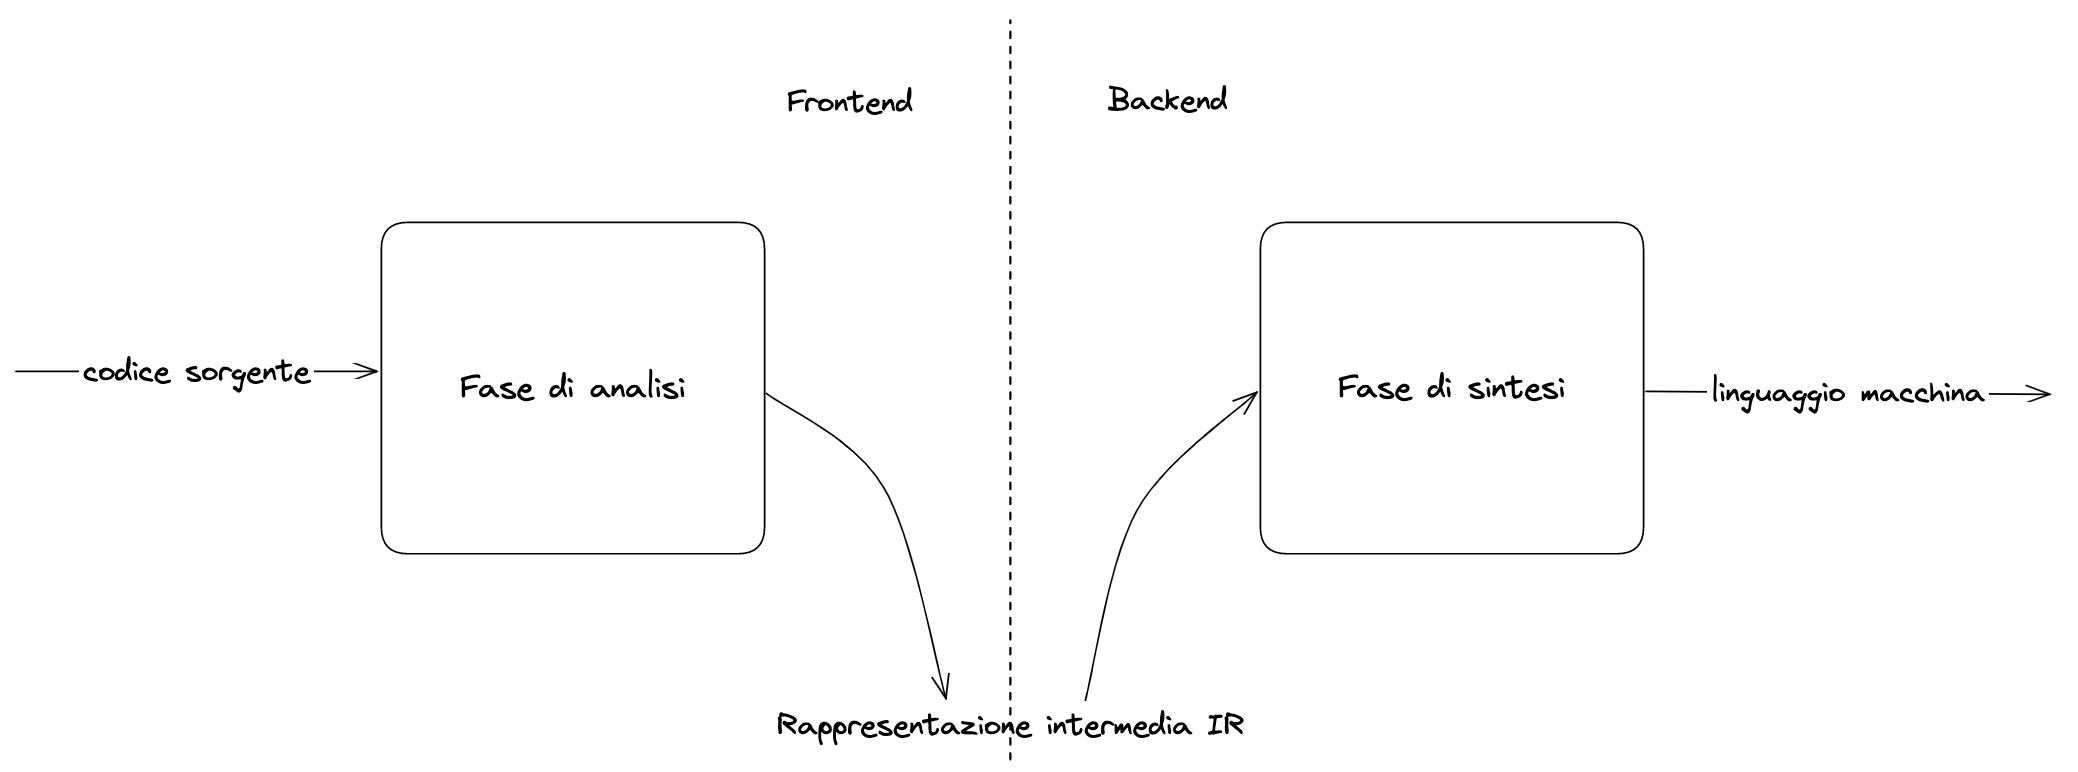
\includegraphics[width=15cm]{./chapters/2.wasi-in-depth/images/7.how_compilers_work.png}
    \label{how_compilers_work_simplified}
    \caption{Una overview sul funzionamento dei compilatori}
\end{figure}

In ambito Wasm, troviamo diverse strategie di compilazione, tra cui JIT (Just In Time) e AOT (Ahead Of Time). I
compilatori JIT traducono il codice Wasm in linguaggio macchina durante l'esecuzione del programma, appena prima che il
codice venga eseguito. Questo significa che il compilatore può ottimizzare il codice in base alle informazioni
disponibili solo a tempo di esecuzione. L'approccio JIT può portare a prestazioni migliori rispetto all'AOT, in quanto
il compilatore ha maggiori informazioni a disposizione per l'ottimizzazione del codice. Tuttavia, la traduzione JIT
richiede una certa quantità di tempo di elaborazione durante l'esecuzione del programma. D'altra parte, i compilatori
AOT traducono il codice Wasm in linguaggio macchina prima dell'esecuzione del programma, solitamente al momento
dell'installazione o del caricamento del modulo. Questo significa che il codice viene tradotto una sola volta, rendendo
l'esecuzione del programma successiva più veloce, poiché il codice già tradotto viene eseguito direttamente. L'approccio
AOT può essere particolarmente utile per applicazioni in cui la velocità di avvio è un fattore critico, come ad esempio
negli ambienti cloud. Tuttavia, la traduzione AOT potrebbe non essere in grado di ottimizzare il codice in modo dinamico
come il compilatore JIT, in quanto non ha informazioni sulle condizioni di esecuzione effettive del programma.

Ci sono vari tipi di compilatori, i più famosi ed usati dai runtime Wasm sono Cranelift e LLVM.
\subsection{Cranelift}
Cranelift\footnote{\url{https://github.com/bytecodealliance/wasmtime/blob/main/cranelift/README.md}} è un compilatore
altamente ottimizzante che è stato progettato specificamente per il bytecode di Wasm. Utilizzando l'IR intermedio CLIF
(Cranelift IR Format), Cranelift è in grado di rappresentare il codice sorgente Wasm in modo strutturato e applicare una
vasta gamma di ottimizzazioni durante la fase di compilazione. CLIF è stato progettato per essere facile da analizzare e
trasformare, consentendo a Cranelift di effettuare una serie di trasformazioni, come la riscrittura di codice per
migliorare le prestazioni o per renderlo più sicuro. Una volta che il codice Wasm è stato tradotto in CLIF, Cranelift
applica una serie di fasi di ottimizzazione dopo le quali, viene convertito in un altro IR intermedio chiamato VCode. Il
VCode è un'astrazione del codice macchina ed è specificatamente legato ad esso, il che significa che descrive le
istruzioni in modo simile a come il processore le esegue, ma a un livello più alto di astrazione. Può essere generato
per diverse architetture, come x86-64, AArch64 (ARM64), RISC-V e IBM z/Architecture. Infine, il VCode viene convertito
in codice macchina specifico per l'architettura di destinazione.

L'utilizzo di due IR intermedie, come CLIF e VCode, consente al compilatore, tramite la prima traduzione, di eseguire
una vasta gamma di ottimizzazioni sul codice sorgente prima della generazione del codice macchina finale. Mentre la
conversione in un secondo IR intermedio, come VCode, permette al compilatore di generare il codice finale specifico per
l'architettura di destinazione, indipendentemente dalla complessità dell'IR intermedio utilizzato per l'ottimizzazione
del codice. 

\subsection{LLVM}
LLVM\footnote{\url{https://llvm.org/}} è un framework di compilazione modulare, che fornisce un insieme di strumenti e
librerie per la compilazione di programmi in diversi linguaggi di programmazione. È molto diffuso ed usato in altri
ambiti al di fuori di Wasm. Analizza e trasforma il codice sorgente in LLVM IR, un linguaggio intermedio di basso
livello che rappresenta il codice sorgente in modo strutturato e indipendente dall'architettura.

Dopo la fase di analisi, LLVM applica diverse fasi di ottimizzazione per migliorare le prestazioni e la sicurezza del
codice generato. Le fasi di ottimizzazione possono essere personalizzate e configurate in modo da ottenere un equilibrio
tra le prestazioni e la complessità del codice generato. Ad esempio, è possibile configurare LLVM per eseguire solo
alcune ottimizzazioni di base per ridurre il tempo di compilazione, oppure è possibile configurarlo per applicare un set
completo di ottimizzazioni per ottenere il massimo delle prestazioni possibili. Una volta completata la fase di
ottimizzazione, LLVM genera codice macchina per l'architettura di destinazione.

\subsection{La differenza}
La differenza principale tra Cranelift e LLVM è nel modo in cui gestiscono l'IR intermedio durante il processo di
compilazione. Cranelift utilizza due IR intermedi, il CLIF, che è stato progettato specificamente per la compilazione di
WebAssembly e il VCode. Invece, LLVM utilizza il suo proprio IR intermedio, che è stato progettato per essere utilizzato
con una vasta gamma di linguaggi di programmazione. Inoltre, mentre Cranelift è stato progettato specificamente per
WebAssembly e supporta solo alcune architetture, LLVM è stato progettato per supportare diverse architetture di
destinazione, tra cui x86, ARM, MIPS, PowerPC, RISC-V e altre. Ciò significa che LLVM può essere utilizzato per
compilare codice sorgente in una vasta gamma di linguaggi di programmazione per diverse architetture di destinazione,
mentre Cranelift è specificamente progettato per compilare codice WebAssembly in alcune architetture specifiche.

\begin{figure}[H]
    \centering
    \captionsetup{justification=centering}
    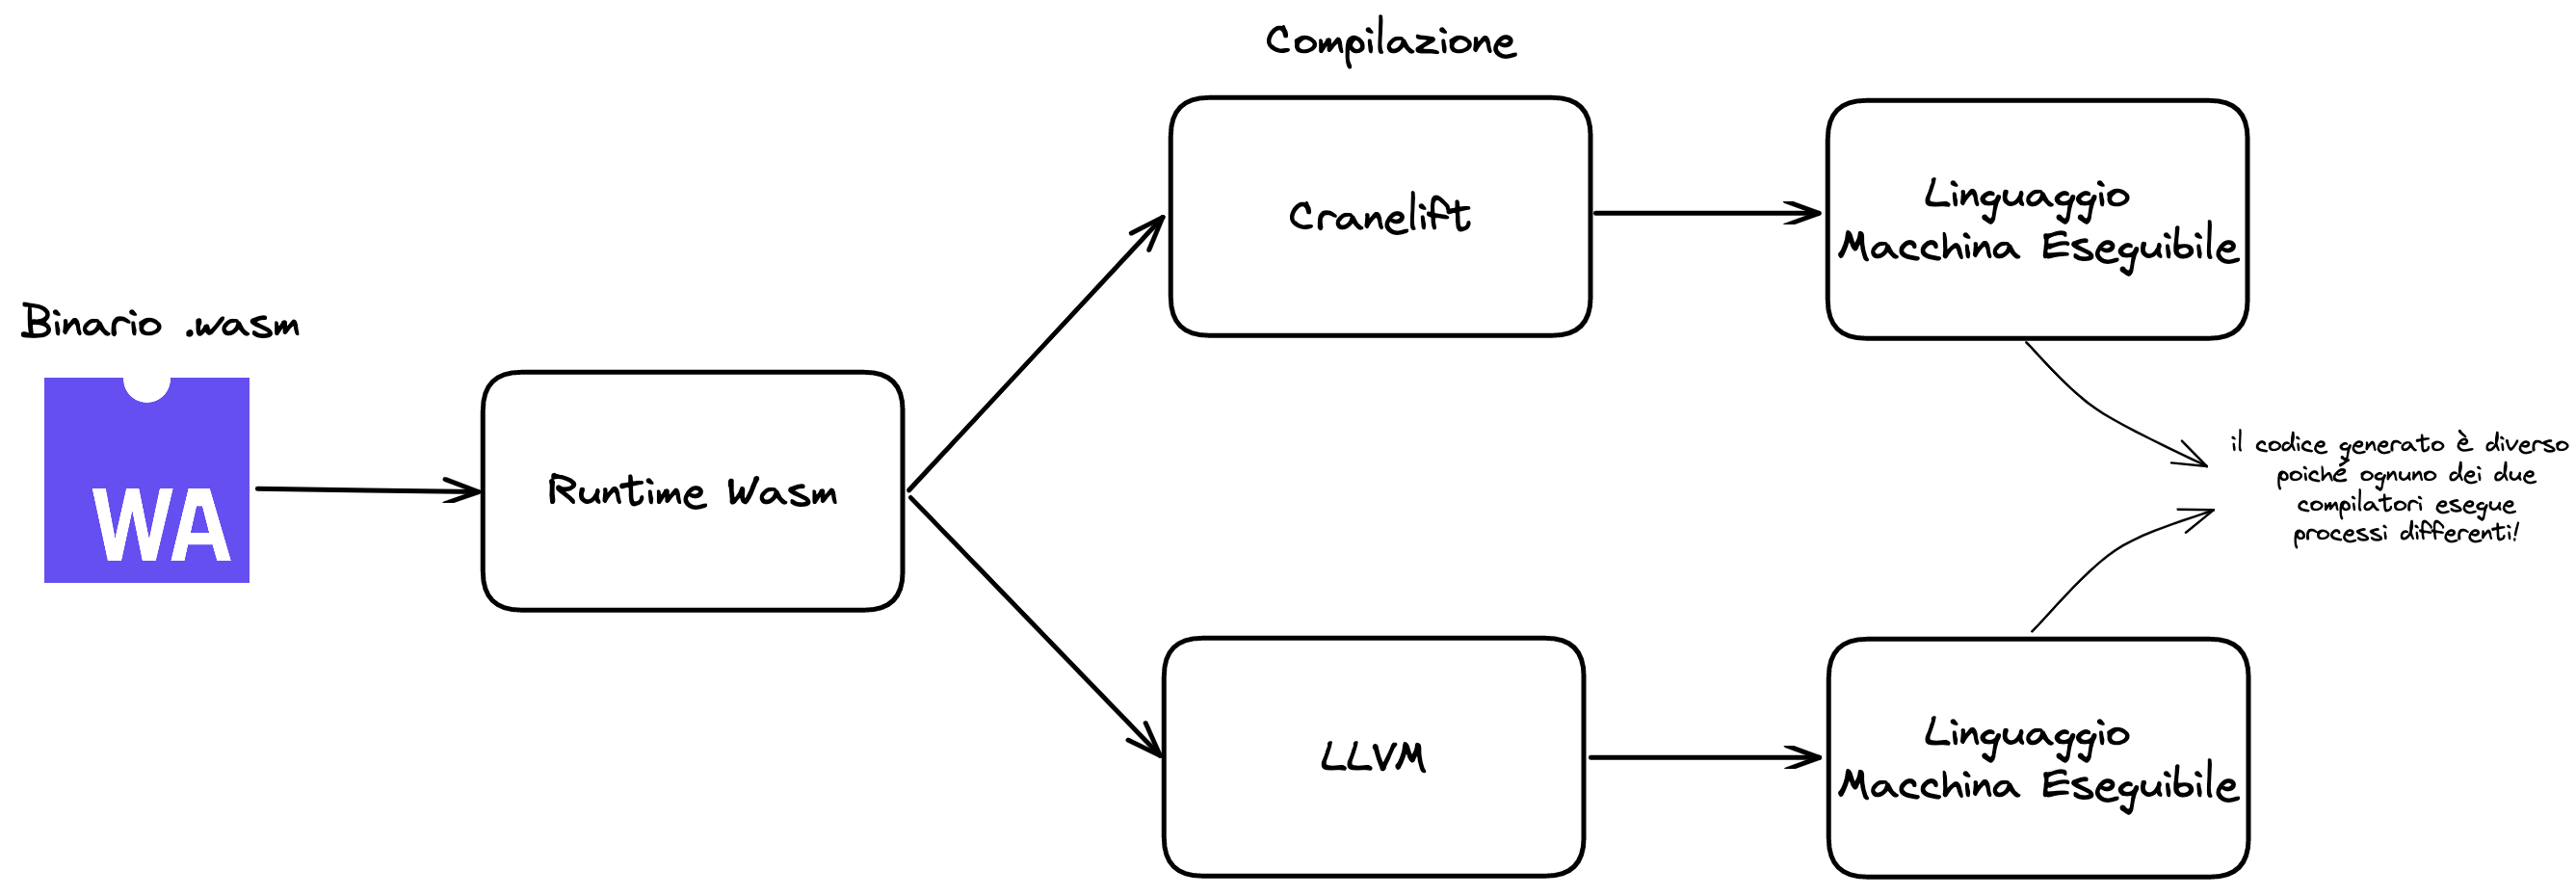
\includegraphics[width=15cm]{./chapters/2.wasi-in-depth/images/11.runtime_to_machine.png}
    \label{runtime_to_machine_code}
    \caption{Dal runtime al linguaggio macchina}
\end{figure}

\subsection{Linguaggi compilati ed interpretati}
Quando si parla di linguaggi di programmazione, sia compilati che interpretati, la creazione di moduli .wasm rappresenta
una sfida diversa per le due realtà. Nel caso dei linguaggi compilati, l'ostacolo principale consiste nel supporto del
compilatore al formato .wasm, che richiede una specifica conoscenza e competenza nel lavorare con questo tipo di
architettura. D'altra parte, per i linguaggi interpretati, la sfida principale è rappresentata dall'interprete stesso,
che deve essere compilato in .wasm per eseguire il codice nativo. Tuttavia, è interessante notare che molti interpreti
dei linguaggi più comuni sono scritti in C/C++, il che rende la compilazione in .wasm più semplice. Pertanto, nella
maggior parte dei casi, i linguaggi interpretati possono essere usati per produrre moduli .wasm senza problemi.

\begin{figure}[H]
    \centering
    \captionsetup{justification=centering}
    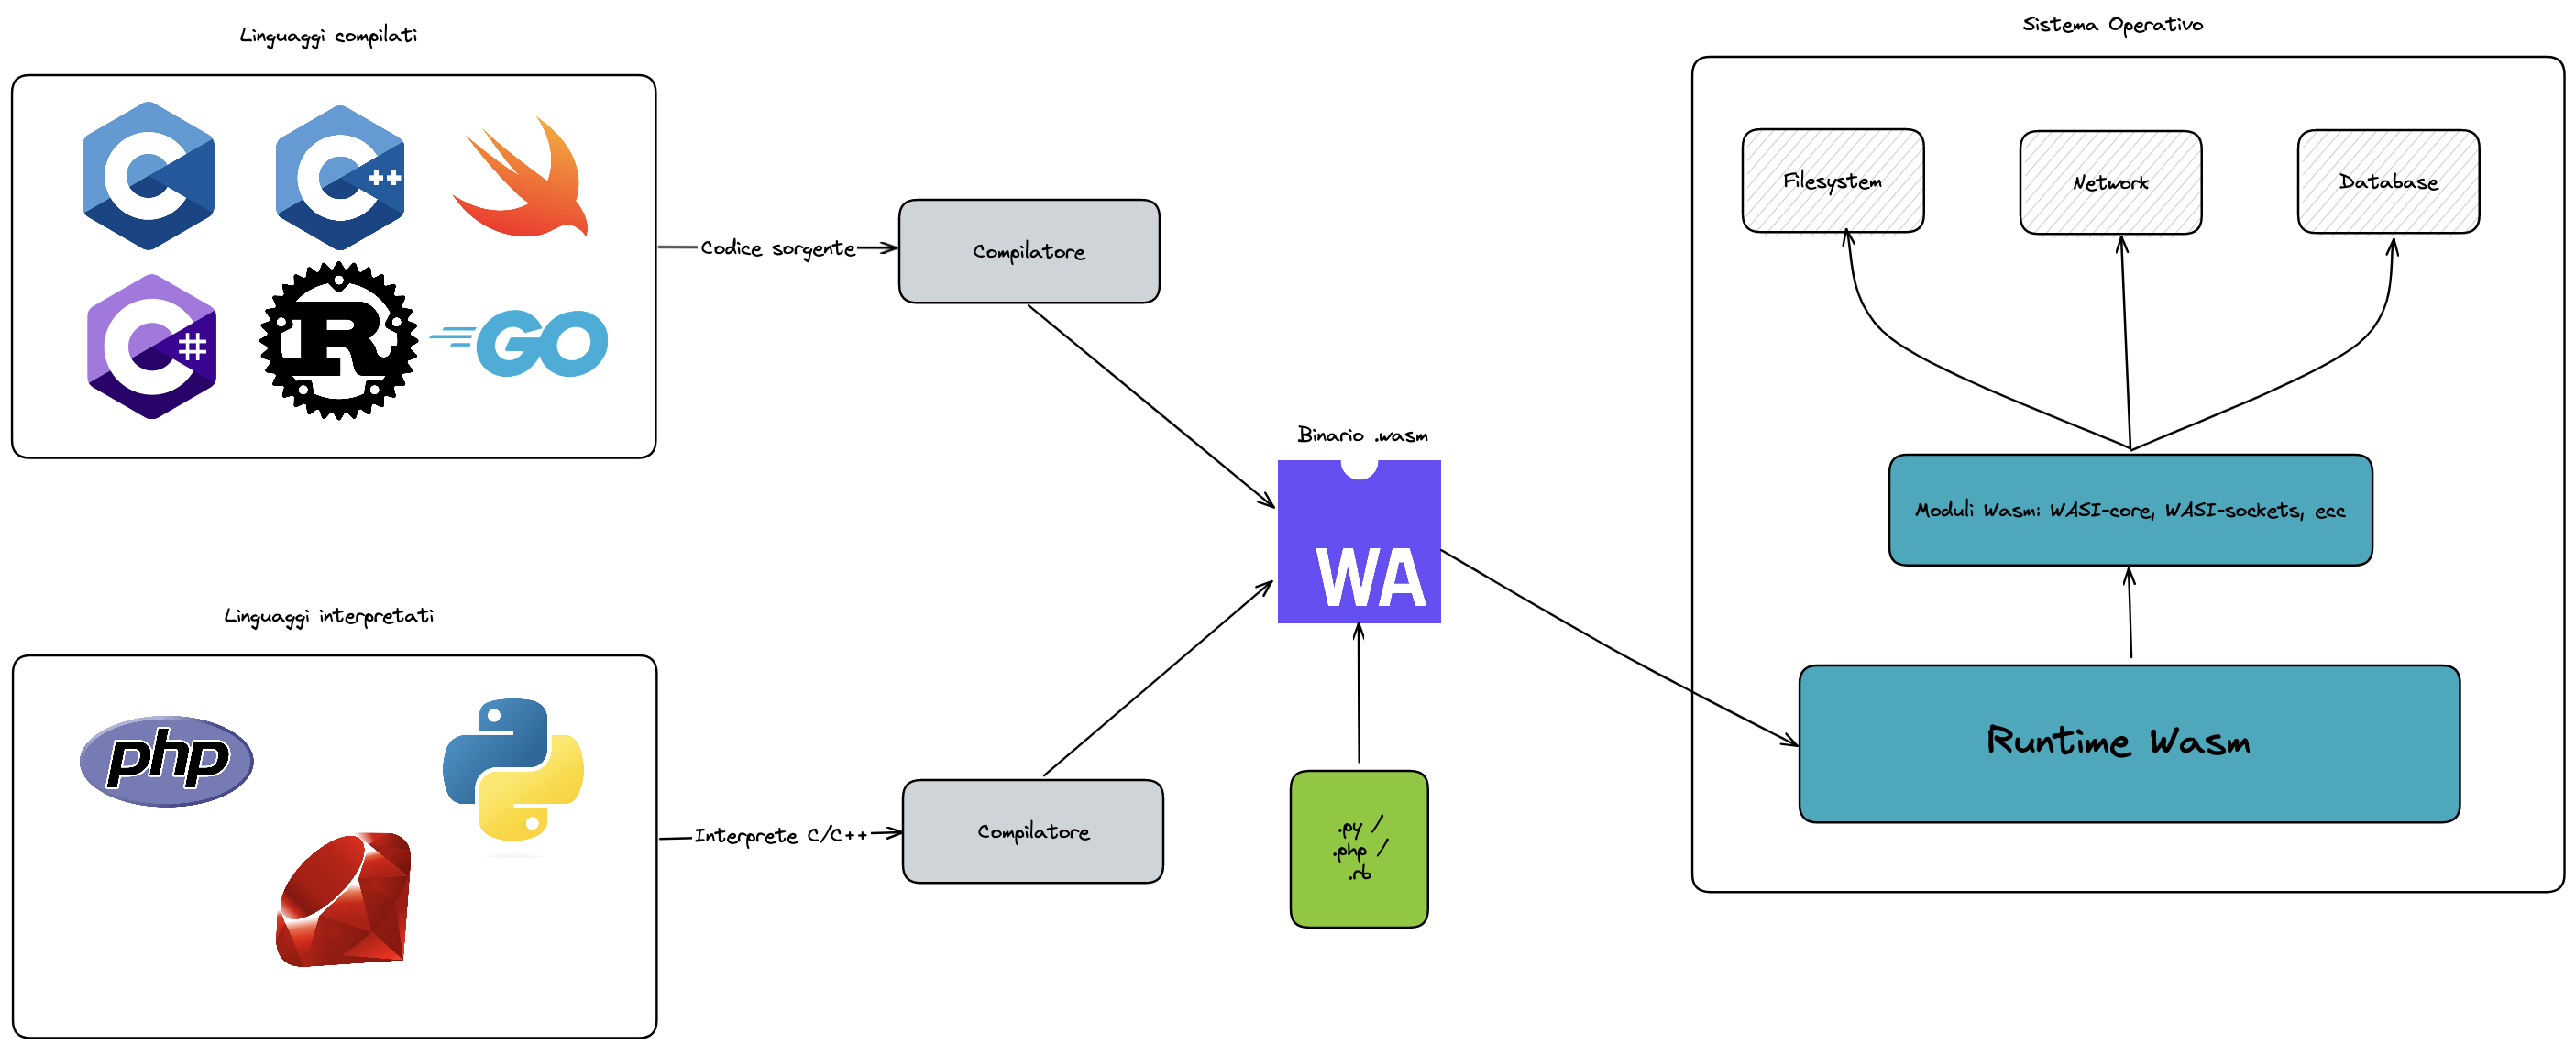
\includegraphics[width=15cm]{./chapters/2.wasi-in-depth/images/9.portability_wasm.png}
    \label{wasm_wasi_portability}
    \caption{Linguaggi compilati e interpretati con Wasm}
\end{figure}

% \section{Il component based model} Al momento della scrittura del documento, diverse interfacce di WASI stanno
% emergendo. Tutte si basano sul WASI-core definito in precedenza e seguono un modello di sviluppo chiamato component base
% model. Il component base model

\section{La gestione delle risorse}
Dopo aver compreso che Wasm è un formato binario di esecuzione compilato da qualsiasi linguaggio di programmazione che
lo supporti, e che WASI è uno standard che definisce interfacce per consentire ai moduli Wasm di comunicare in modo
sicuro ed isolato dal sistema sottostante, ci concentriamo ora sul motivo per cui vengono definiti container leggeri e
considerati la terza ondata del cloud computing.

Il cloud computing ha subito due evoluzioni significative. La prima ha visto il passaggio dalla gestione manuale dei
server offrenti servizi alla creazione di macchine virtuali che ha permesso di ridurre i costi e la manutenzione dei
servizi, garantendo l'isolamento delle applicazioni. Siccome una VM è essenzialmente un intero sistema operativo con
all'interno diversi package, dati e applicazioni, occupa molti GB di memoria e non è adatta per essere scalata in modo
veloce in quanto il boot time è nell'ordine dei secondi-minuti.

Poi c'è stato l'avvento delle immagini Docker e dei relativi container. I container sono un'unità software relativamente
leggera e portatile che esegue le applicazioni in modo isolato, ma condividendo il kernel del sistema operativo
sottostante. Ciò significa che, a differenza delle macchine virtuali, non richiedono l'esecuzione di un intero sistema
operativo all'interno di un altro sistema operativo, il che rende la creazione e l'istanziazione molto più veloce
rispetto alle VM; funzionalità che ha portato all'ascesa di strumenti di orchestrazione come
Kubernetes\footnote{\url{https://kubernetes.io/docs/home/}} che si occupa di gestire i carichi del sistema e di scalare
automaticamente le applicazioni per garantire una risposta efficiente alle richieste in arrivo. Inoltre, i container
offrono un'ulteriore vantaggio in quanto possono essere facilmente interconnessi tramite Docker Compose, strumento che
permette di organizzare i container in gruppi logici e interconnetterli in modo veloce e affidabile, semplificando
notevolmente la gestione di applicazioni complesse composte da diversi componenti.

Per fare un esempio concreto, un'immagine Docker è composta da un sistema operativo leggero come Alpine Linux,
all'interno del quale viene installata l'applicazione desiderata e le sue dipendenze. Quando si avvia un container,
viene effettuato il boot di questo sistema operativo, vengono caricate le dipendenze e infine si esegue l'applicazione.

Si può quindi evincere che:
\begin{itemize}
    \item Un'immagine docker è un intero filesystem
    \item Ogni immagine ha un sistema operativo: esistono immagini Linux e immagini Windows, non immagini generiche
    \item L'immagine docker dipende dall'architettura sottostante; un Mac con processore ARM può solo eseguire immagini
    compilate per ARM
    \item Le applicazioni devono tener conto del sistema operativo e dell'architettura dell'immagine Docker su cui
    verranno eseguite
\end{itemize}

Una tipica immagine Docker è più leggera di un'intera VM e tende anche ad usare meno risorse rispetto ad essa. Tuttavia
possono arrivare facilmente a dimensioni nell'ordine delle centinaia di MB e dei GB.

\begin{figure}[h]
    \centering
    \captionsetup{justification=centering}
    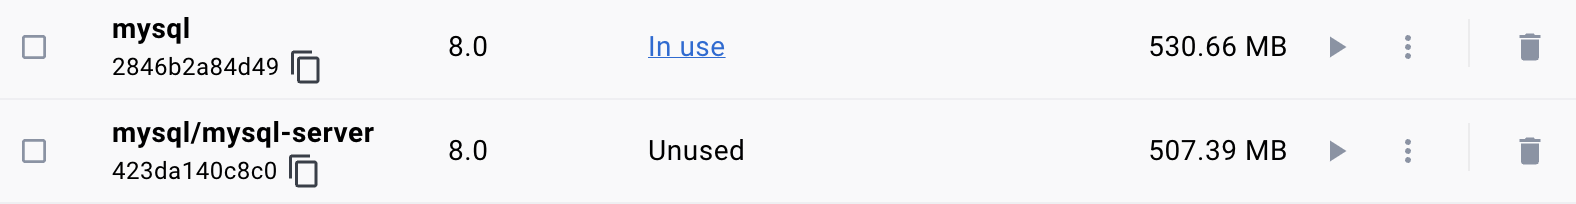
\includegraphics[width=15cm]{./chapters/2.wasi-in-depth/images/8.docker-images-size.png}
    \label{mysql_docker_image}
    \caption{Esempio di immagine Docker per mysql}
\end{figure}

WebAssembly invece viene definito come un container leggero poiché migliora il concetto dei container. Una delle ragioni
che lo rende così leggero è il fatto che, a differenza delle immagini Docker, un modulo Wasm non richiede di essere
inserito all'interno di un mini sistema operativo. Inoltre, grazie al suo formato neutrale, con l'ausilio di WASI, può
essere eseguito su qualsiasi macchina supportata dal runtime utilizzato, che si occupa di gestire l'interazione,
l'isolamento e il caricamento di tutte le risorse necessarie per il modulo.

\subsection{Docker+Wasm}
Di recente, Docker ha introdotto il supporto ai container Wasm\cite{docker-wasm-tech-preview}, costituendo così un
notevole passo avanti per l'adozione di Wasm nel mondo cloud. Grazie alla sua diffusione, Docker rende più agevole la
distribuzione dei container. Tuttavia, i container Wasm su Docker operano in maniera leggermente differente rispetto ai
container tradizionali.

In genere, su Docker, l'avvio e l'esecuzione dei container avviene tramite Containerd, un runtime di container open
source che funge da interfaccia tra il demone Docker e i container. Quando viene eseguito un comando Docker come "docker
run", il demone Docker comunica con Containerd per avviare un nuovo container. Containerd si occupa di gestire l'avvio e
l'esecuzione dei container, compresa la creazione del filesystem, l'assegnazione di namespace di sistema isolati e
l'aggiunta di eventuali opzioni di rete. Quando il container viene avviato, Containerd lo esegue in una sandbox,
proteggendo il sistema host da eventuali problemi che potrebbero verificarsi all'interno del container. Per eseguirlo
viene utilizzato Runc, un runtime di container che implementa lo standard Open Container Initiative (OCI). Questo viene
eseguito all'interno di un "container shim", un piccolo processo che funge da ponte tra Runc e Containerd. Il container
shim svolge il compito di trasferire i comandi tra Containerd e Runc, gestendo inoltre eventuali segnalazioni di errorri
tra i due processi. Questa divisione dei ruoli è necessaria per garantire che il container venga eseguito in modo
isolato dal resto del sistema.

La principale differenza tra un container tradizionale e uno Wasm risiede nella loro architettura. Infatti, mentre un
container tradizionale necessita di un sistema operativo leggero e dipende dal kernel dell'host per funzionare, uno Wasm
è basato su un'architettura sandboxed e isolata gestita da un runtime. Ciò significa che i container Wasm non richiedono
un sistema operativo gestito all'interno del container, ma sono semplicemente composti da un modulo .wasm, il che li
rende più leggeri. Per eseguire un container Wasm su Docker, è necessario utilizzare una versione modificata del
containerd-shim chiamata containerd-wasm-shim che è versione appositamente progettata per gestire l'architettura sandbox
di Wasm e serve da ponte tra Docker e WasmEdge, che è il runtime Wasm utilizzato per eseguire l'applicazione al posto di
Runc.
\begin{figure}[h]
    \centering
    \captionsetup{justification=centering}
    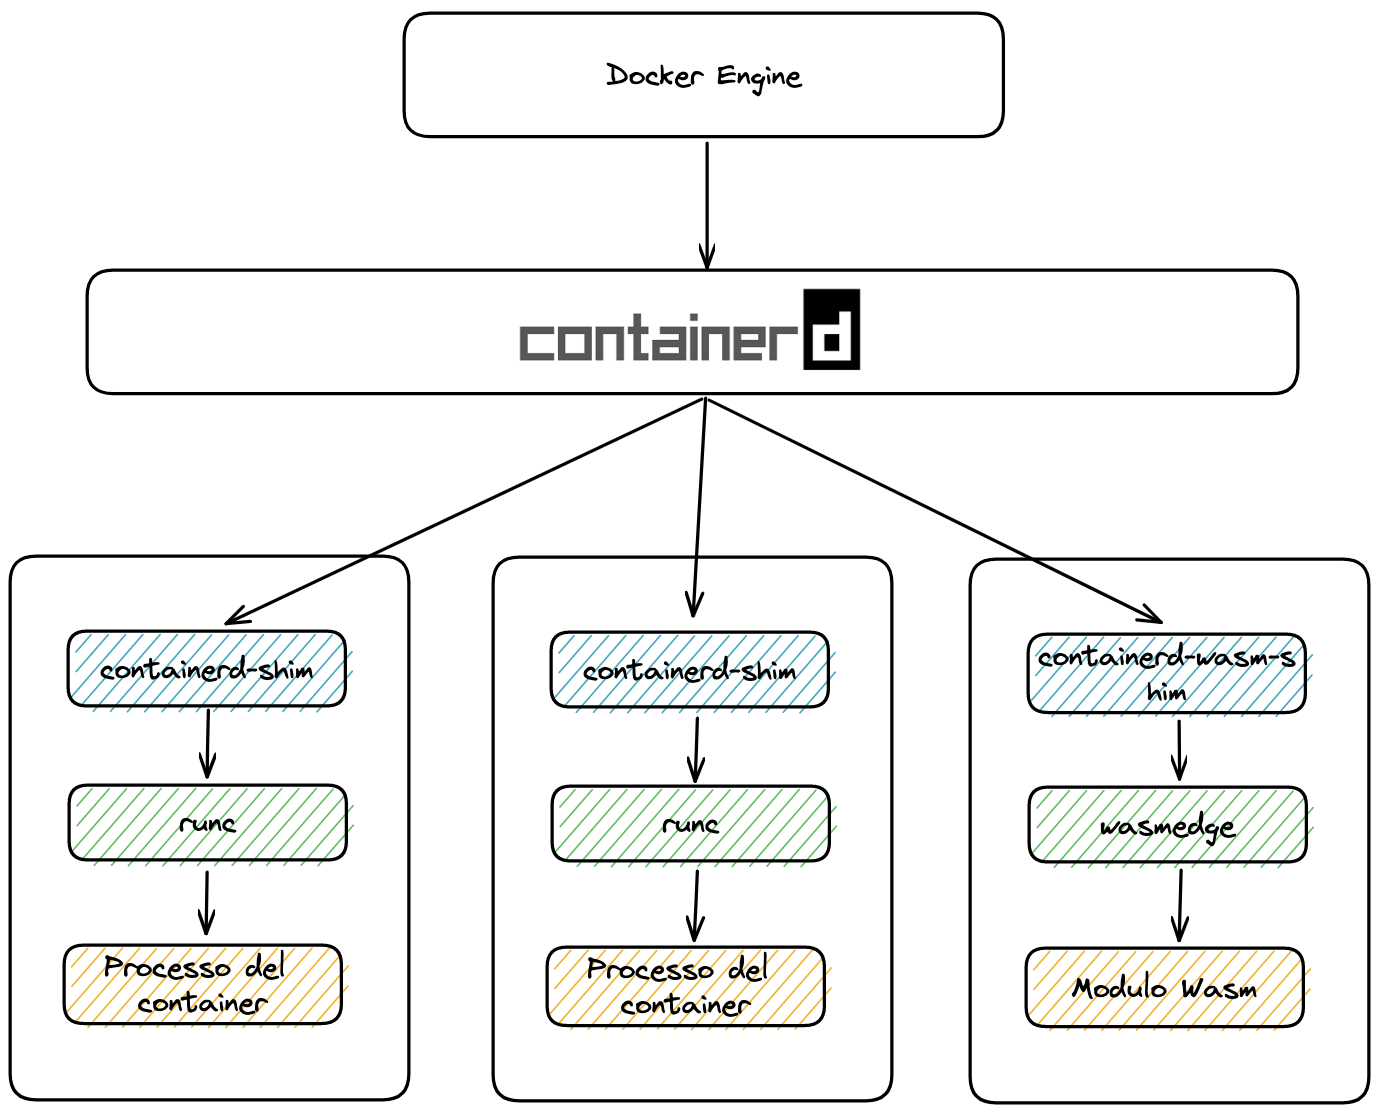
\includegraphics[width=8cm]{./chapters/2.wasi-in-depth/images/10.docker_and_wasm.png}
    \label{docker_and_wasm_wasmedge}
    \caption{Container tradizionali e container Wasm su Docker}
\end{figure}

\subsubsection{Wasm al posto di Docker?}
Viene da chiedersi a questo punto se Wasm prenderà il sopravvento su Docker\cite{why-containers-and-wasm}. In generale
possiamo dire di no, entrambi hanno i loro punti di forza e debolezza. I container sono utili in quei contesti in cui la
portabilità è importante ma si vuole anche mantenere un forte controllo sul sistema mentre Wasm permette lo sviluppo di
applicazioni sicure di default con pochissimo overhead aggiuntivo. Si possono intendere come tecnologie complementari,
che in alcuni contesti possono coesistere come vedremo nel terzo capitolo del documento.

\subsection{Uno use case: i microservizi con Wasm}
\subsubsection{Il problema}
Consideriamo ora Wasm in uno scenario reale: quello dei microservizi\cite{a-way-to-rethink-microservices} riprendendo
la spiegazione fornita riguardante la sicurezza in WASI. Nella costruzione di un applicazione è ormai la norma
utilizzare codice scaricato da internet attraverso i package manager. Questo può causare non pochi problemi di
sicurezza, soprattutto se si tiene conto del fatto che ogni pacchetto richiede a sua volta altre dipendenze per
funzionare. Prendiamo come esempio NodeJS, dove per creare un'applicazione ad architettura a microservizi, potremmo
utilizzare il framework ExpressJS per aggiungere le funzionalità necessarie, come il routing, il middleware, la gestione
dei file, l'integrazione dei database, e così via. Tuttavia, questo significherebbe anche installare tutte le dipendenze
utilizzate da ExpressJS, che potrebbero essere circa un centinaio. Prima di iniziare a scrivere una sola riga di codice
avremmo già importato migliaia di altre righe di codice che potrebbero presentare vulnerabilità. Poi, per eseguire il
nostro servizio, avremmo bisogno di un server HTTP che andrebbe eseguito per ogni microservizio e che avrebbe bisogno di
rimanere sempre in ascolto di nuove connessioni. Nel caso di un servizio particolarmente utilizzato, avremmo anche
bisogno di duplicare le istanze del microservizio per gestire il traffico. Tutto questo comporterebbe un aumento dei
costi, poiché più pesante è il nostro codice, maggiori le risorse necessarie in termini di storage e utilizzo della CPU.
Inoltre, la maggior parte del tempo, a meno di un servizio super trafficato, staremo probabilmente pagando per un
servizio in esecuzione, anche se in idle, replicato.

L'adozione di questa metodologia comporta l'acquisizione di un debito tecnico prima ancora di iniziare a scrivere una
sola riga di codice. Infatti, installando le dipendenze che gestiscono il core della nostra applicazione, come il server
HTTP, l'implementazione TLS e l'interazione con il sistema sottostante, ci troviamo a dover gestire la sicurezza
dell'intero sistema ospitante, inclusi i permessi corretti nel sistema. Inoltre, se dovesse emergere una vulnerabilità
di sicurezza in una di queste dipendenze, saremo costretti a risolverla da soli, poiché un fix potrebbe non essere
disponibile in tempi brevi. Fortunatamente, nel corso degli anni sono state sviluppate soluzioni come le PaaS o le IaaS,
in grado di gestire e alleviare gli sviluppatori dal fardello di questa gestione low-level.

Tuttavia, queste soluzioni sono spesso dipendenti dai provider cloud di turno, i quali effettuano scelte in base alle
proprie necessità. Ad esempio, un servizio PaaS come AWS Elastic Beanstalk può differire dall'omonimo Google App Engine,
entrambi servono scopi simili ma con modalità differenti.

\subsubsection{La soluzione}
Wasm offre una soluzione in grado di eliminare la necessità di interagire con il sistema ospitante, il web server HTTP,
il livello TLS e così via. Queste operazioni sono comuni a tutti i web framework, indipendentemente dal linguaggio di
programmazione utilizzato, che sia questo Javascript, Rust o Java. Grazie a Wasm, possiamo concentrarci sulle
funzionalità della nostra applicazione, senza dover gestire l'infrastruttura sottostante e la sua comunicazione con
essa. Anche se le dipendenze introdotte nell'applicazione sono ancora a carico nostro, sarebbe il runtime sottostante a
gestire gran parte del lavoro in quanto ci garantirebbe l'isolamento e la sicurezza dell'esecuzione. Inoltre, la nostra
applicazione con Wasm può scalare veramente a zero, poiché un solo server HTTP gestito dal runtime sarebbe in grado di
redirigere le richieste al servizio adatto con tempi di risposta rapidi in quanto i nostri microservizi non sono altro
che minuscoli binari .wasm. Combiniamo queste caratteristiche al fatto che Wasm ci permette di usare il linguaggio di
programmazione che vogliamo e abbiamo una tecnologia estremamente versatile per quanto riguarda lo sviluppo in cloud.

Il terzo capitolo metterà un focus proprio su questi concetti appena introdotti per dimostrare l'effettivo valore di
Wasm in ambiente cloud.

\section{La sicurezza con WASI}
% WASI segue il 'principle of least privilege' e il 'capability-based security model'.
\subsection{Il problema}
\label{sec:security-problem}
Nell'ambito dello sviluppo software, l'utilizzo di librerie esterne è diventato una pratica comune per facilitare la
creazione di applicazioni complesse. Queste librerie open source, disponibili sotto forma di pacchetti software, sono
facilmente accessibili tramite l'uso di appositi strumenti chiamati package manager. I package manager sono strumenti di
gestione del software che consentono di gestire, salvare e distribuire le librerie di codice necessarie alla creazione
di un'applicazione. Inoltre, consentono di installare automaticamente tutte le dipendenze richieste per far funzionare
un software, semplificando notevolmente il processo di integrazione di nuove funzionalità all'interno di
un'applicazione. Con l'utilizzo di un package manager, gli sviluppatori possono concentrarsi maggiormente sullo sviluppo
di funzionalità specifiche, piuttosto che sulla gestione delle dipendenze.
\begin{figure}[h]
    \centering
    \captionsetup{justification=centering}
    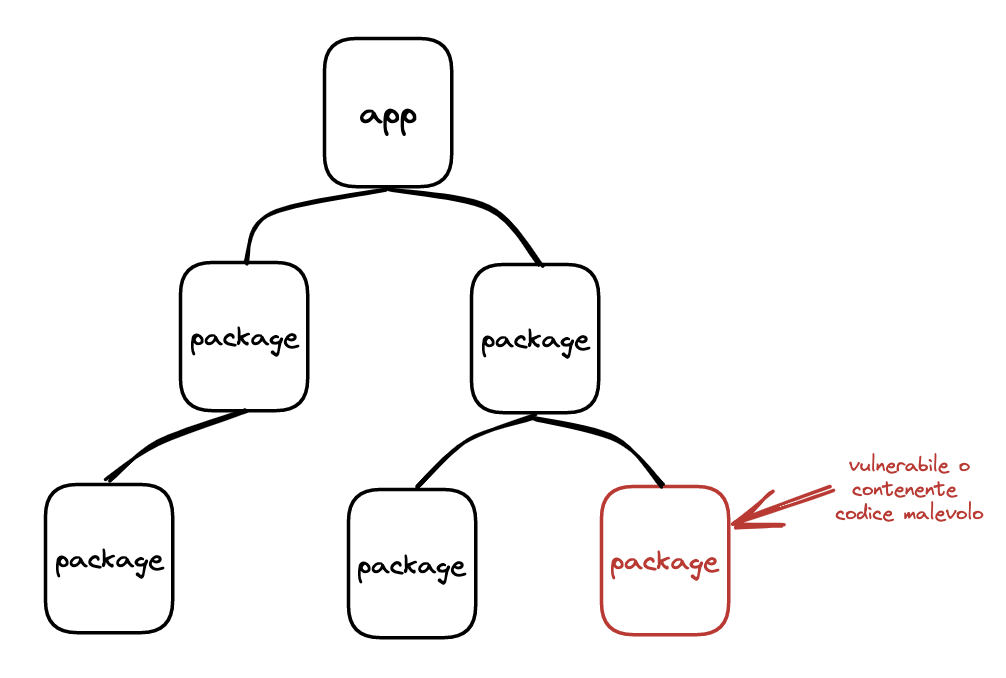
\includegraphics[width=8cm]{./chapters/2.wasi-in-depth/images/1.malicious_or_vuln_code.png}
    \label{app_package}
    \caption{Come sono composte le applicazioni moderne}
\end{figure}
In questo modo, è possibile ridurre il lavoro necessario per la creazione di applicazioni complesse, migliorare
l'efficienza del processo di sviluppo e aumentare la qualità del software prodotto. D'altra parte, questo modello di
sviluppo espone le applicazioni ad una grossa problematica, cosa succederebbe se in uno di questi pacchetti software ci
fosse inserito codice malevolo o codice vulnerabile? Purtroppo non è uno scenario remoto:
\begin{quote}
    The average application development project has 49 vulnerabilities and 80 direct dependencies (open source code
    called by a project); \\
    \textit{Snyk 2022 State of Open Source Security Report}\cite{snyk-2022-open-source-security}
\end{quote}
Per peggiorare le cose, non tutte queste vulnerabilità vengono risolte, si stima che solo il 59\% dei pacchetti software
risolva le vulnerabilità trovate e in media ci impieghi circa 110
giorni\footnote{\url{https://snyk.io/reports/open-source-security}}.
% \footnote{\url{https://snyk.io/reports/open-source-security\#Open-source-vulnerabilities-are-becoming-harder-to-fix}}.
\begin{figure}[h]
    \centering
    \captionsetup{justification=centering}
    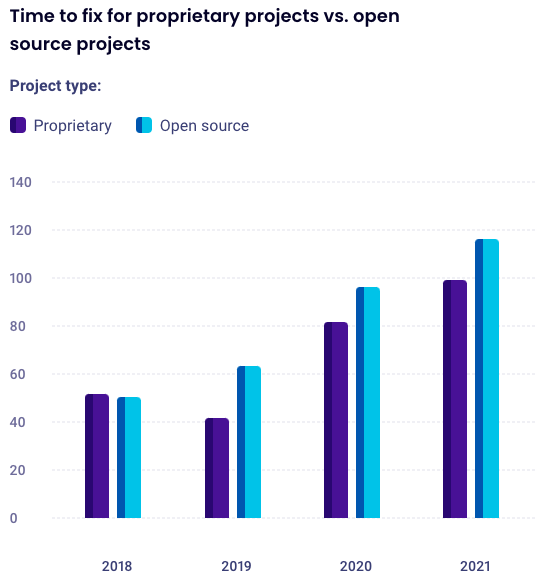
\includegraphics[width=12cm]{./chapters/2.wasi-in-depth/images/12.time_to_fix_os_sec.png}
    \label{time_to_fix_security}
    \caption{Tempo necessario per risolvere le vulnerabilità, un confronto tra open source e codice proprietario}
\end{figure}
\subsection{Una possibile soluzione}
Esistono diverse strategie che gli sviluppatori possono adottare per proteggere il loro software e gli utenti finali. Ad
esempio, si potrebbe utilizzare uno scanner per controllare le applicazioni e le dipendenze, tuttavia questa soluzione
non è sempre efficace, poiché gli scanner sono facilmente aggirabili. Un'altra opzione potrebbe essere quella di
registrarsi ad un servizio che notifichi gli sviluppatori delle vulnerabilità trovate nel codice, ma anche questa
soluzione presenta delle limitazioni, in quanto potrebbe non individuare tutte le vulnerabilità presenti nel software.
Infine, un'altra strategia possibile sarebbe quella di revisionare il codice ogni volta che si fa un update delle
dipendenze, ma questa soluzione potrebbe funzionare solo per progetti piccoli con poche dipendenze, mentre per progetti
più grandi e complessi potrebbe risultare impraticabile. Queste soluzioni esistenti cercano di individuare le
vulnerabilità del software, ma non offrono una vera e propria prevenzione. La soluzione ideale sarebbe quella di
prevenire tali vulnerabilità alla radice, ma è più facile a dirsi che a farsi. E se avessimo un modo per limitare le
applicazioni e i loro package in modo che siano confinati dentro ad una sorta di contenitore chiuso che non permetta di
disturbare le altre applicazioni del sistema e quindi di causare danni? Possiamo farlo attraverso molti modi, molti dei
quali sono già stati affrontati in passato. \\
Partiamo nel capire come due applicazioni non si interferiscono durante la loro esecuzione. È una soluzione che esiste
fin dai primi sistemi operativi. La soluzione adottata è affidare al sistema operativo il compito di proteggere e
controllare l'esecuzione delle applicazioni tramite l'utilizzo dei "processi". Quando una nuova applicazione viene
avviata, il sistema operativo crea un nuovo processo con un'area di memoria dedicata, che non può accedere alle aree
riservate degli altri. Se ha bisogno di comunicare con altri, deve prima richiedere il permesso e farlo tramite le pipe.
\begin{figure}[H]
    \centering
    \captionsetup{justification=centering}
    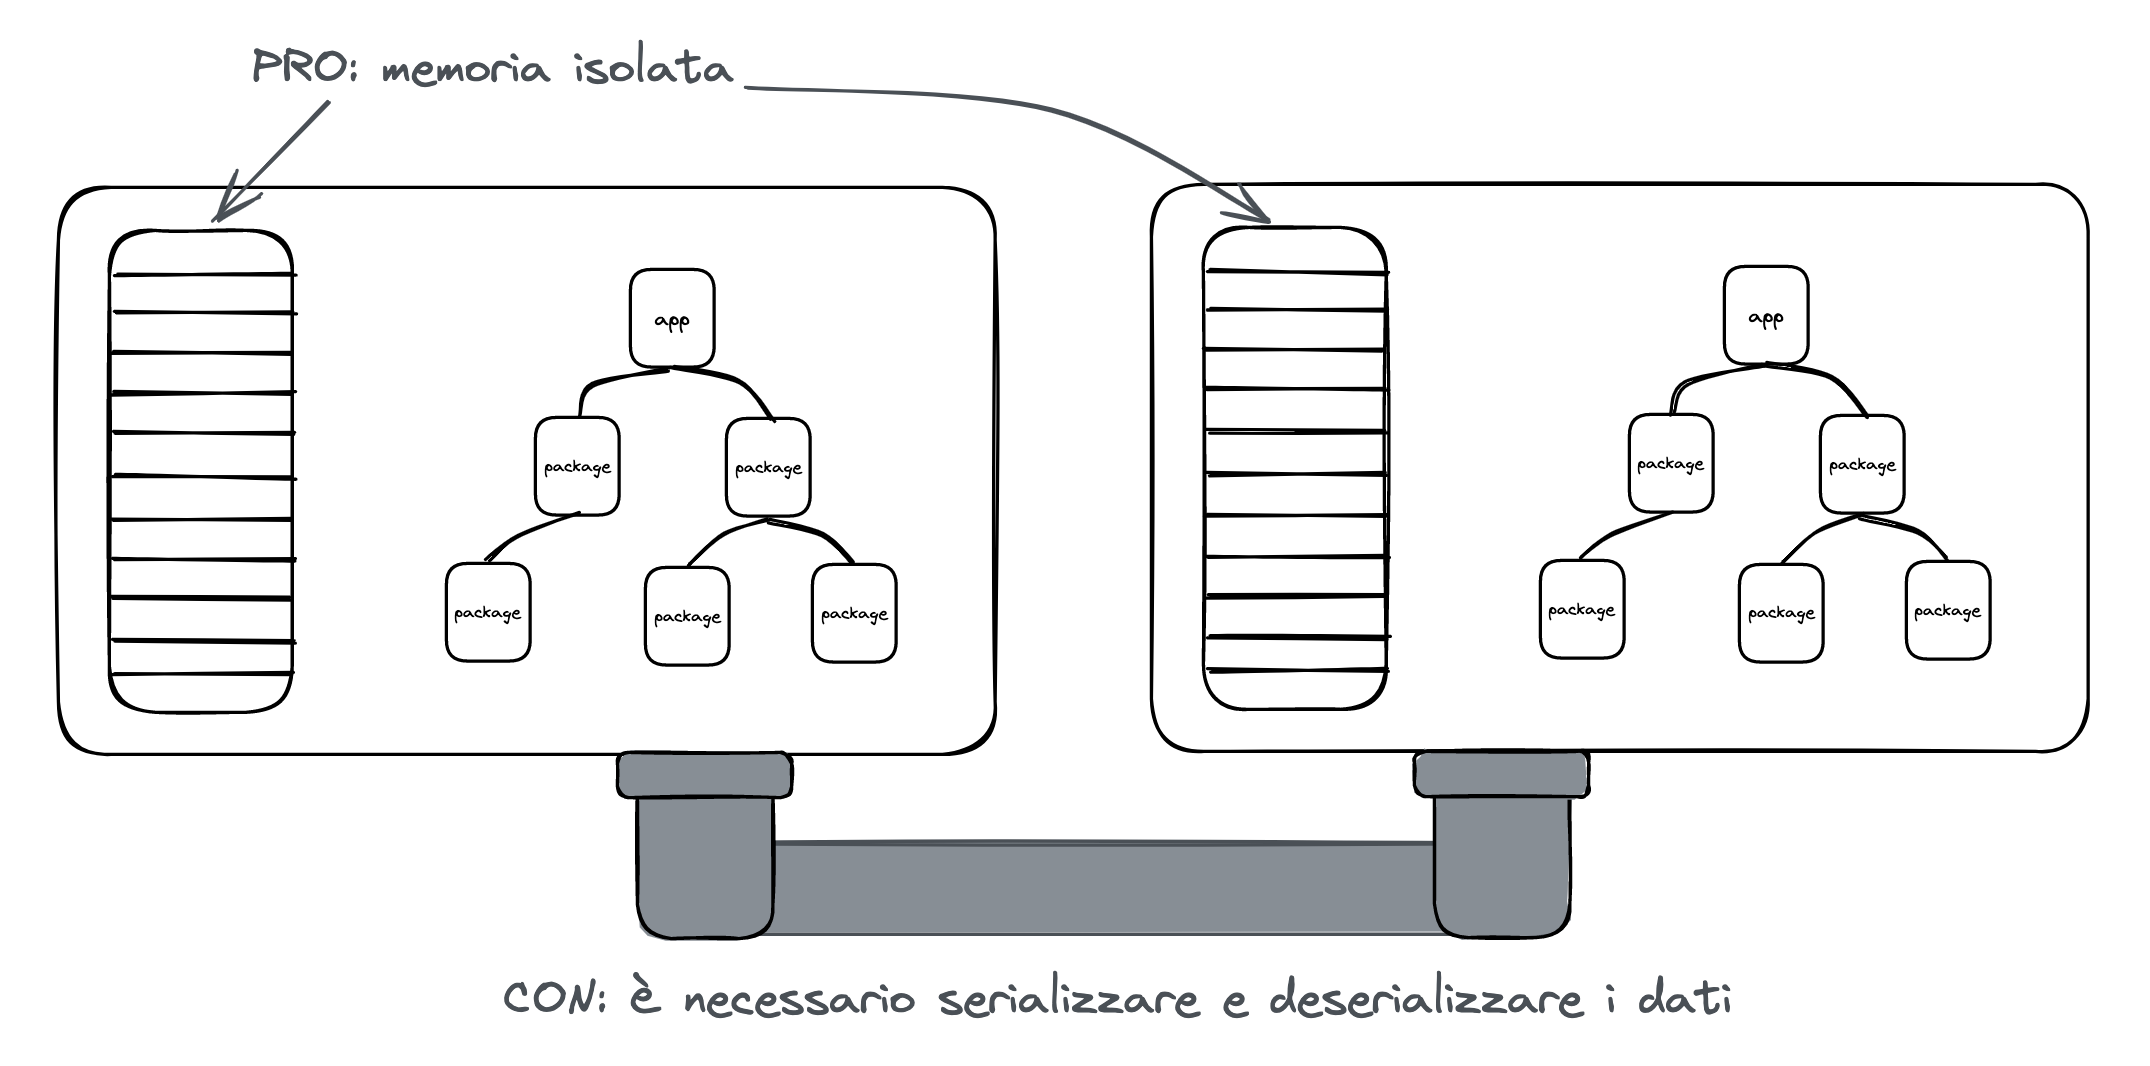
\includegraphics[width=10cm]{./chapters/2.wasi-in-depth/images/2.process_isolation.png}
    \label{process_isolation}
    \caption{Isolamento dei processi nei sistemi operativi}
\end{figure}
Questo sistema risolve il problema della condivisione della memoria a runtime ed evita che un eventuale applicazione
manipoli la memoria di altri, ma non garantisce, ad esempio, che non possa accedere al filesystem per effettuare qualche
operazione non prevista.\\ 
Le VM e i container sono stati sviluppati in origine proprio per questo motivo, garantiscono che un'applicazione in
esecuzione in una VM o container non possa accedere al filesystem di altri degli altri in esecuzione sulla stessa
macchina. Questo però non risolve del tutto un'altro problema, l'applicazione in un container o in una VM è comunque in
grado di accedere al proprio sistema e causare danni al suo interno. Se volessimo proprio vietare anche determinate
azioni all'interno di uno stesso sistema? Con il modello sandbox, potremmo farlo isolando le applicazioni, rimuovendo
l'accesso alle API e alle system call su questo. Potremmo perciò arrivare alla conclusione che per garantire la
sicurezza e l'isolamento di ogni package sia necessario isolarlo all'interno della propria sandbox. Ciò però
risulterebbe inefficiente in quanto porterebbe presto ad un esaurimento delle risorse del sistema ed introdurrebbe un
overhead nella comunicazione tra le componenti dell'applicazione.
\begin{figure}[H]
    \centering
    \captionsetup{justification=centering}
    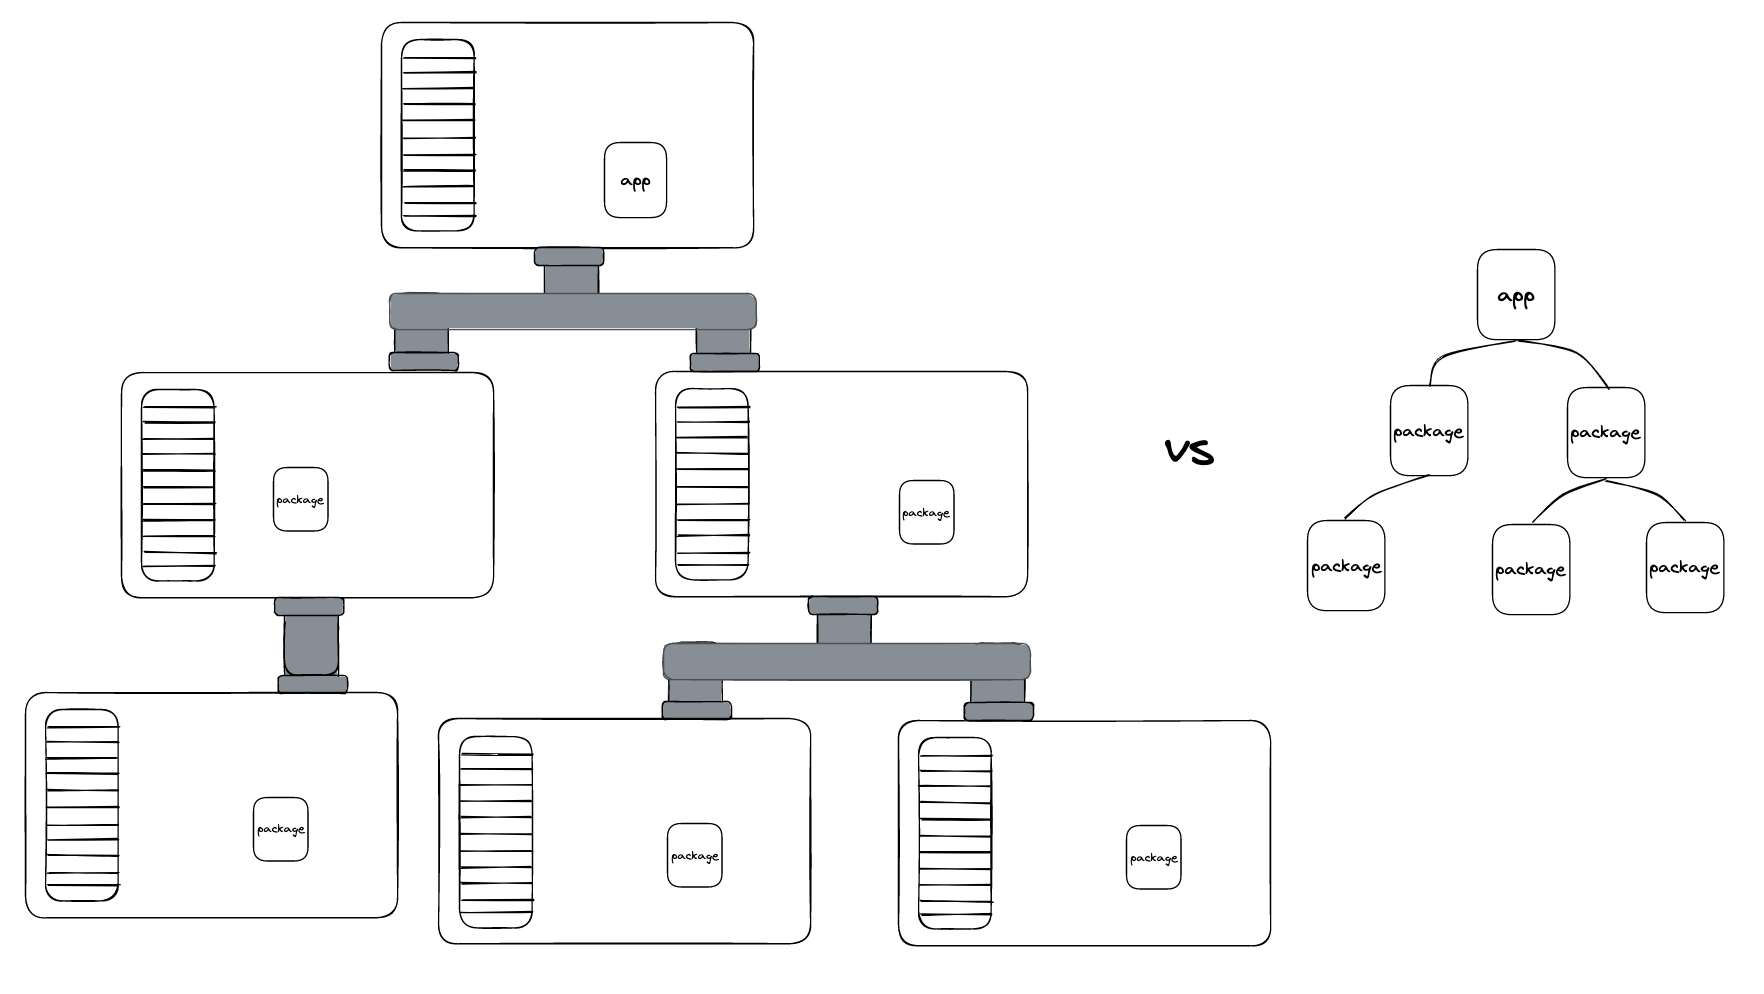
\includegraphics[width=10cm]{./chapters/2.wasi-in-depth/images/3.package_isolation_processes.png}
    \label{process_package_in_sandbox}
    \caption{Isolamento dei package in sandbox isolate, evidente inefficienza e overhead}
\end{figure}
Come facciamo quindi a garantire l'isolamento di ogni package senza esaurire le risorse del sistema?
\subsection{La soluzione: i nanoprocessi di WebAssembly}
WebAssembly offre un'efficace forma di isolamento che previene al codice di operare a proprio piacimento, i
nanoprocessi\cite{wasm-nano-processes}. I nanoprocessi sono strutture simili ai processi standard di Unix ma che
risultano essere più leggeri e di dimensioni ridotte. Risiedono all'interno di un ambiente di esecuzione chiamato
sandbox, che rappresenta un processo contenitore isolato dall'esterno. La memoria a cui ogni nanoprocesso ha accesso è
uno slice della memoria della  sandbox e per accedere ai dati di un altro modulo deve avere l'autorizzazione esplicita
per farlo. Questa autorizzazione viene passata in modo gerarchico, dall'alto verso il basso a partire dalla sandbox che
a sua volta ha ricevuto i permessi all'avvio. In questo modo, la sandbox coordina l'accesso ai dati e garantisce che
ogni nanoprocesso operi in modo indipendente e sicuro, senza che eventuali package vulnerabili possano causare danni
all'esterno. L'uso di nanoprocessi consente di ottimizzare le prestazioni dell'applicazione, evitando costose chiamate
di sistema e semplificando la comunicazione tra i vari moduli Wasm.
\begin{figure}[h]
    \centering
    \captionsetup{justification=centering}
    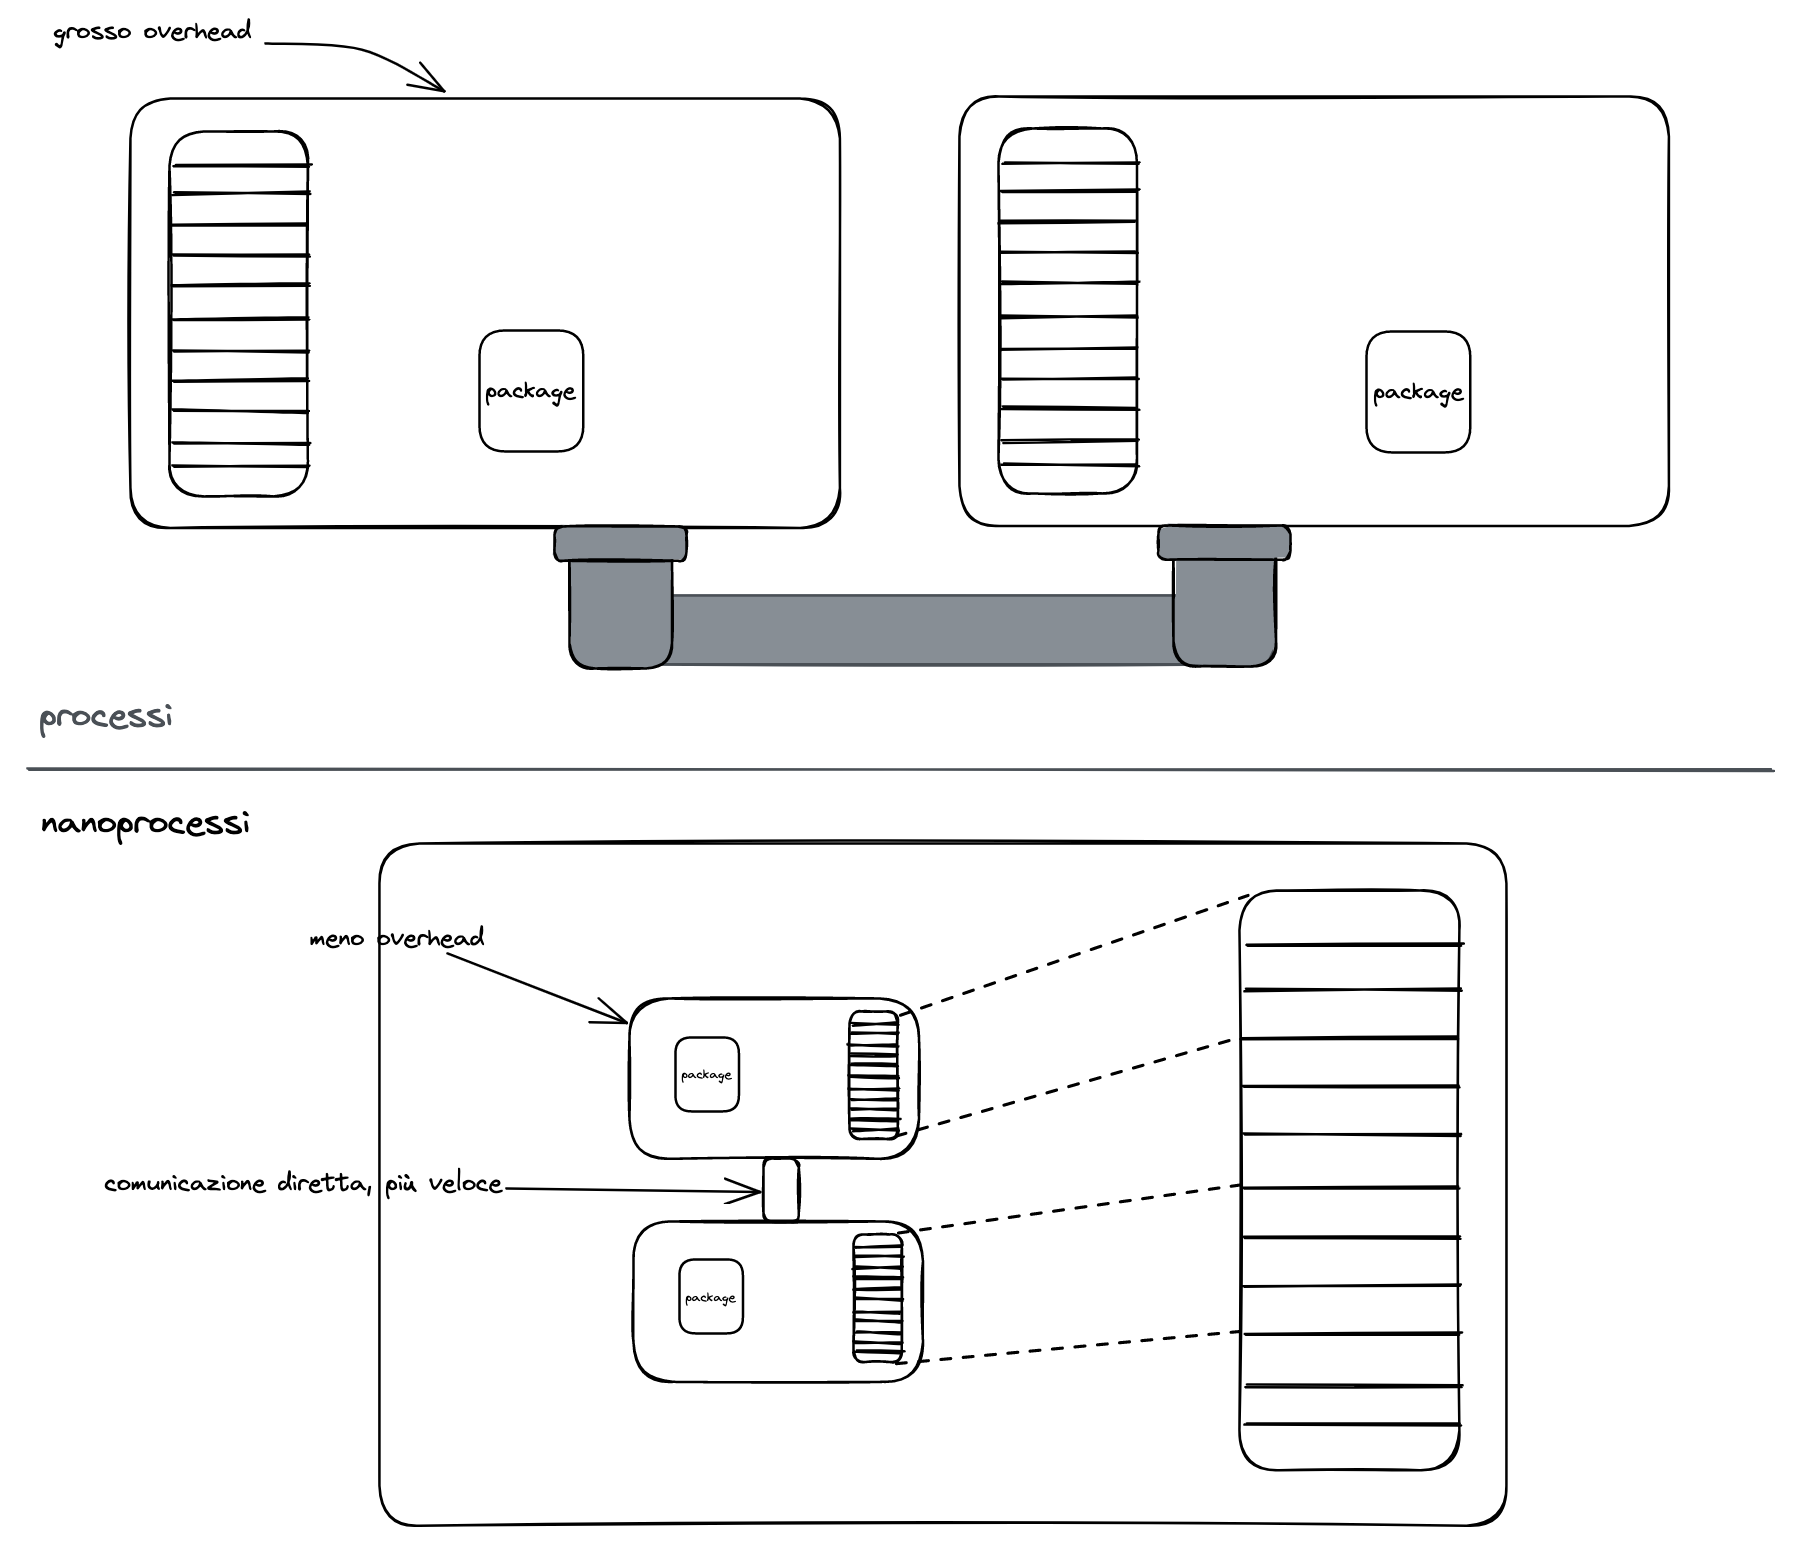
\includegraphics[width=10cm]{./chapters/2.wasi-in-depth/images/4.nanoprocesses.png}
    \label{nanoprocesses}
    \caption{Nanoprocessi di Wasm}
\end{figure}
\\
Tutte le caratteristiche di WebAssembly descritte finora rendono questa tecnologia una soluzione sicura per l'esecuzione
di codice al di fuori del browser. Per esempio, se del codice malevolo tentasse di accedere a un file su cui la sandbox
non ha i permessi, il modulo WebAssembly verrebbe interrotto sollevando un'eccezione e il processo terminerebbe con un
errore. Inoltre, anche se la sandbox avesse i permessi per accedere a un determinato file, questi permessi potrebbero
non essere associati al modulo contenente il codice malevolo e anche in questo caso il processo verrebbe interrotto. In
relazione al codice vulnerabile, sarebbe estremamente difficile per un attaccante trovare un modulo che abbia sia
l'autorizzazione a utilizzare una determinata system call sia l'autorizzazione su un determinato file nel filesystem.

% \subsection{Interazione tra i nanoprocessi}


\subsection{Capability Based Model}
Il modello basato sulle capacità è un approccio alla sicurezza informatica che mira a garantire la protezione dei
sistemi mediante la concessione di autorizzazioni specifiche, chiamate "capacità", ai processi del sistema. Questo
modello è stato concepito per la prima volta negli anni sessanta\cite{capability-based-security} e si basa su tecniche
di sviluppo che mirano ad assegnare privilegi minimi\cite{Saltzer1975ThePO} ai processi per consentire loro di eseguire
solo le operazioni necessarie per svolgere il loro compito specifico. È un'alternativa alle ACL (Access Control
List)\cite{samarati2001access} che sono un metodo di controllo degli accessi basato su liste di controllo degli accessi,
dove ogni oggetto (come file, cartelle, stampanti, ecc.) ha una lista di controllo degli accessi associata che contiene
una serie di voci per specificare quali utenti o gruppi hanno il permesso di accedere all'oggetto e quali tipi di
accesso sono consentiti (come lettura, scrittura, esecuzione, ecc.). In un modello di sicurezza basato su capability,
ogni processo ha un insieme di capacità specifiche che gli consentono di accedere alle risorse del sistema. Una capacità
non è altro che una chiave di autorità, associata ad un particolare oggetto. Possiamo pensarla come un indice che punta
ad una tupla\cite{wasm-capability-tuple} (x, r), dove x è l'oggetto ed r è l'insieme dei diritti d'accesso su di esso.
Ad esempio, se la tupla (file1, \{leggi, scrivi\}) è associata ad un processo tramite una reference mantenuta da questo,
tale processo può leggere e scrivere sul file1, ma non può eseguire altre azioni su di esso. Quando un processo deve
accedere all'oggetto, può farlo senza richiedere l'autorizzazione al sistema operativo, in quanto il possesso della
capability (la reference) rappresenta già l'autorizzazione per farlo. In un modello basato sulle capabilities, il
sistema operativo non è responsabile del controllo delle autorizzazioni per i processi, ma piuttosto della gestione
della lista di capabilities disponibili e della prevenzione di eventuali modifiche non autorizzate.
\subsubsection{Un esempio}
\label{sec:capability-example}
Supponiamo che un processo abbia in memoria il seguente path:
\begin{lstlisting}
    /etc/shadow
\end{lstlisting}
Questo rappresenta il nostro oggetto x della tupla e supponiamo poi di aver associato all'oggetto anche il diritto di
lettura r: 
\begin{lstlisting}
    O_RDWR
\end{lstlisting}
Così da avere la tupla (/etc/shadow, O\_RDWR). Questa non rappresenta ancora la capability per il processo di accedere
all'oggetto poiché non si può verificare l'autorità su di esso. Ipotizziamo ora di avere anche il file descriptor per
tale file.
\begin{lstlisting}
    int fd = open("/etc/shadow", O_RDWR);
\end{lstlisting}
La variabile fd contiene l'indice di un descrittore di file presente nella tabella dei descrittori di file del processo
e ciò rappresenta la capability dell'oggetto a cui si sta accedendo. La presenza di questo descrittore nella tabella dei
descrittori è sufficiente per garantire che il processo abbia accesso legittimo all'oggetto. \\

WASI adotta il modello di Nuxi CloudABI\footnote{\url{https://github.com/NuxiNL/cloudabi}}, che unisce i concetti di
POSIX e del modello capability based. In questo modello, ogni risorsa del sistema, come file, directory e socket, è
identificata da un file descriptor UNIX-like, che rappresenta la capability su un certo oggetto del sistema. Ciò
significa che un processo non può accedere a tale oggetto se non è in possesso della capability adatta. Per esempio,
WASI non permette l'accesso alla system call open() che restituisce un file descriptor, ma al contrario, utilizza la
opennat system call, che richiede un file descriptor precedentemente aperto, ovvero la capability associata.
Essenzialmente quindi, un modulo Wasm potrà interagire, ad esempio con il filesystem, solo se la sandbox gli fornirà in
precedenza le capabilities necessarie su di una certa directory all'avvio. Questi file descriptor saranno aperti in
anticipo dalla sandbox tramite la \hyperref[sec:libpreopen]{Libpreopen} e passati ai moduli Wasm quando necessario.
\subsubsection{Il modello in azione: un esempio}
Per comprendere meglio questo modello, possiamo analizzare
un'applicazione\footnote{\url{https://github.com/ilcors-dev/bachelor-thesis/blob/main/prototypes/1.file/src/main.rs}}
scritta in Rust\footnote{\url{https://www.rust-lang.org/}} che si occupa di copiare dei file del filesystem da una
posizione ad un'altra. Per eseguire il modulo Wasm generato dalla compilazione del codice sorgente, utilizzeremo il
runtime Wasmtime.
\begin{figure}[h]
    \centering
    \captionsetup{justification=centering}
    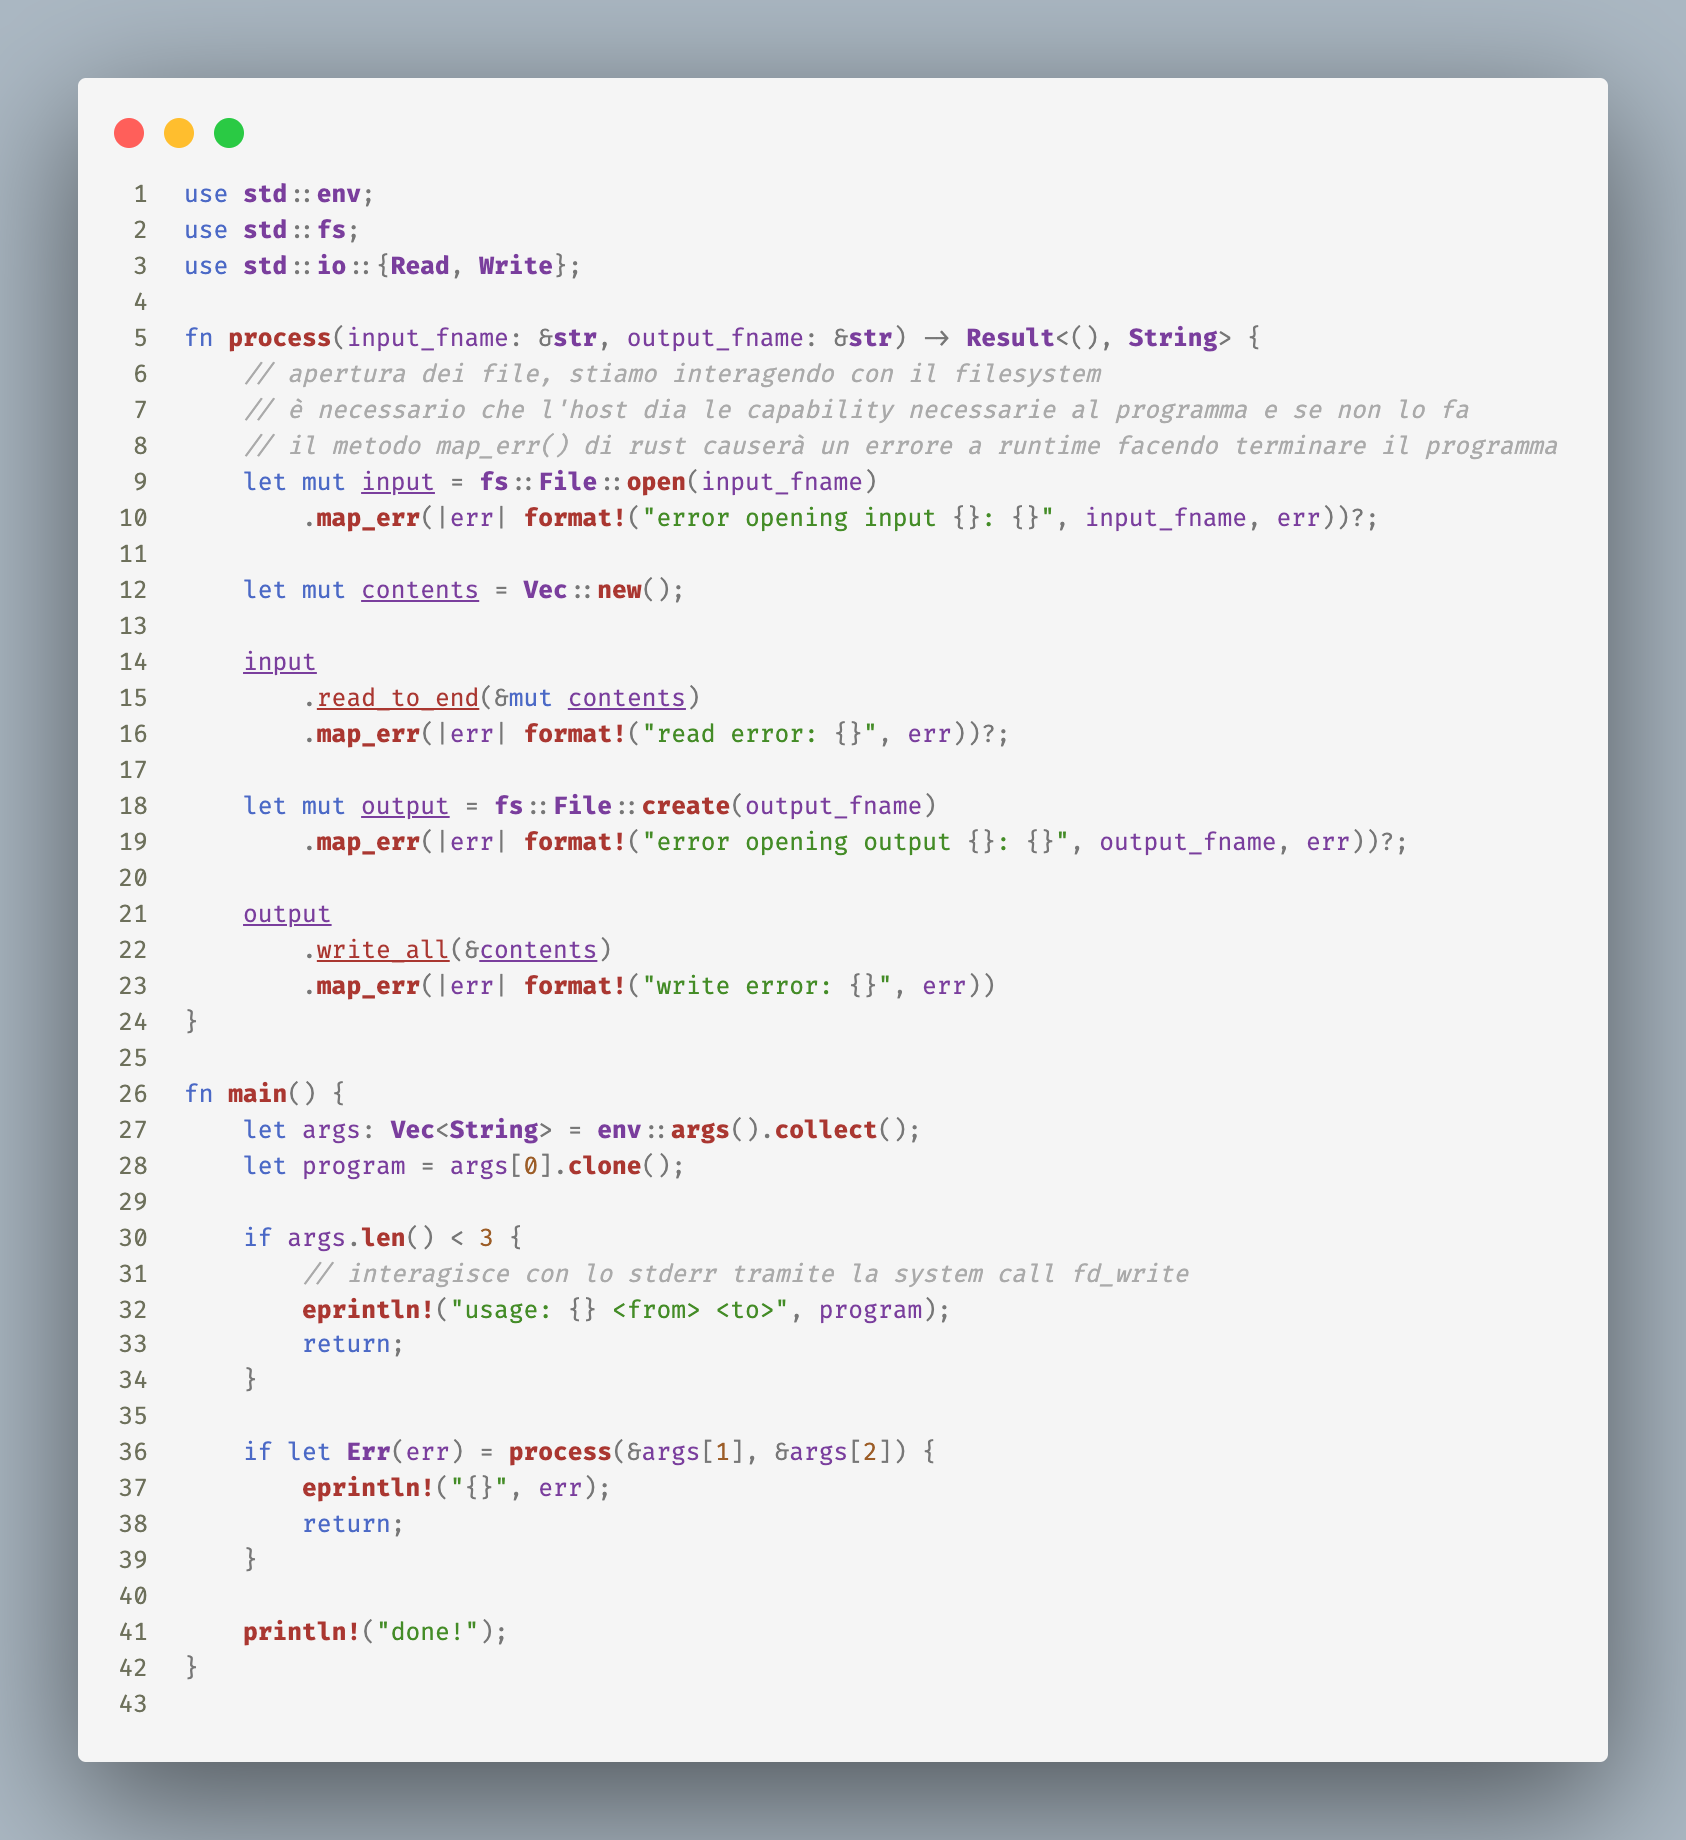
\includegraphics[width=15cm]{./chapters/2.wasi-in-depth/images/5.wasi_capability_example.png}
    \label{wasi_capabilities_example}
    \caption{Il modello capability based in azione}
\end{figure}
Compiliamo il programma tramite cargo, il gestore di pacchetti predefinito di Rust.
\begin{lstlisting}
    cargo build --target wasm32-wasi
\end{lstlisting}

E proviamo ad eseguirlo senza garantire le capability necessarie tramite.

\begin{lstlisting}
    wasmtime target/wasm32-wasi/debug/file.wasm tocopy.txt /tmp/out.txt
    error opening input tocopy.txt: failed to find a pre-opened file descriptor through which "tocopy.txt" could be opened
\end{lstlisting}
Cosa è andato storto? Analizzando l'errore, si evince che il programma sta tentando di aprire un file chiamato
'tocopy.txt', ma non dispone del file descriptor corrispondente necessario. In altre parole, Wasmtime non ha fornito le
capability adatte per consentire all'applicazione di eseguire la copia del file. \\
Proviamo invece ora a fornire le giuste capability in questo modo:
\begin{lstlisting}
    wasmtime --dir=. --dir=/tmp target/wasm32-wasi/debug/file.wasm tocopy.txt /tmp/out.txt
    done!
\end{lstlisting}
Analizziamo cosa è successo. L'opzione --dir istruisce Wasmtime di pre-aprire la cartella corrente '.' e la cartella di
destinazione '/tmp' rendendole entrambi disponibili al programma. Quando l'applicazione chiama la funzione File::open
sta effettivamente chiamando la system call open() passando come parametro il path del file. In questo frangente
interviene la WASI libc, che in modo trasparente, traduce il path in un path relativo a quello già pre-aperto in
precedenza da Wasmtime utilizzando la libreria \hyperref[sec:libpreopen]{Libpreopen}. \\In questo modo WASI è in grado
di adottare il modello capability based e portarlo a livello di system call senza che il programma in sè debba essere
modificato in qualche modo particolare.

È importante anche notare che, di default, la sandbox non espone la variabile d'ambiente \$PWD all'applicazione
WebAssembly, la directory corrente va pertanto passata attraverso un path relativo. Infatti:
\begin{lstlisting}
    wasmtime --dir=\$PWD --dir=/tmp target/wasm32-wasi/debug/file.wasm tocopy.txt /tmp/out.txt
    error opening input tocopy.txt: failed to find a pre-opened file descriptor through which "tocopy.txt" could be opened
\end{lstlisting}

Parlando di directory corrente con '.', cosa succede con i '..', ovvero i path traversal? Funzionano? Sappiamo che in
applicazioni tradizionali la sanificazione dell'input è a carico dello sviluppatore, mentre con WASI?

\begin{lstlisting}
    wasmtime --dir=. --dir=/tmp target/wasm32-wasi/debug/file.wasm tocopy.txt /tmp/../etc/passwd
    error opening output /tmp/../etc/passwd: failed to find a pre-opened file descriptor through which "/tmp/../etc/passwd" could be opened
\end{lstlisting}

Come possiamo notare l'applicazione viene bloccata prima di raggiungere il sistema operativo, infatti l'errore non
riguarda gli eventuali permessi necessari per accedere ad /etc/passwd, bensì parla della mancanza di capacità necessaria
per effettuare l'operazione. Le applicazioni WASI non hanno possibilità di accedere a file al di fuori delle directory
esplicitamente garantite dalla sandbox!

Ciò si traduce in applicazioni molto più sicure di default grazie alla riduzione della superficie di attacco
disponibile.


\printbibliography

\end{document}